%%%%%%%%%%%%%%%%%%%%%%%%%%%%%%%%%%%%%%%%%%%%%%%%%%%%%%%%%%%%%%%%%%%%%%%%%%%%%%%%%%%
% THE BEER-WARE LICENSE (Revision 42):                                            %
% <r@twopi.eu> schrieb diese Datei. Solange Sie diesen Vermerk nicht entfernen,   %
% können Sie mit dem Material machen, was Sie möchten. Wenn wir uns eines Tages   %
% treffen und Sie denken, das Material ist es wert, können Sie mir dafür ein Bier %
% ausgeben. Robert Hemstedt                                                       %
%%%%%%%%%%%%%%%%%%%%%%%%%%%%%%%%%%%%%%%%%%%%%%%%%%%%%%%%%%%%%%%%%%%%%%%%%%%%%%%%%%%

\documentclass[12pt,a4paper]{article}
\usepackage[utf8x]{inputenc}
%\usepackage{ucs}
\usepackage[left=2.0cm, right=2.0cm, top=2.0cm, bottom=2.0cm]{geometry}
\usepackage{amsmath}
\usepackage{amsfonts}
\usepackage[ngerman]{babel}
\usepackage{bbm}
\usepackage{amssymb}
\usepackage[amsthm,thmmarks]{ntheorem}
%\usepackage{tabularx}
\usepackage[arrow, matrix, curve]{xy}
\usepackage{graphicx}
% b) Lemma, Satz, Theorem usw.
\makeatletter
\renewtheoremstyle{plain}%
  {\item[\hskip\labelsep \theorem@headerfont ##1\ ##2:]}%
  {\item[\hskip\labelsep \theorem@headerfont ##1~##2~##3:]\mbox{}}
\makeatother

\theoremstyle{plain}
\newtheorem{Theorem}{Theorem}[section]
\newtheorem{Satz}[Theorem]{Satz}
\newtheorem{Prop}[Theorem]{Proposition}
\newtheorem{Lemma}[Theorem]{Lemma}
\newtheorem{Korollar}[Theorem]{Korollar}
\newtheorem{Definition}[Theorem]{Definition}
\newtheorem*{Folgerung}[Theorem]{Folgerung}
\newtheorem*{Behauptung}[Theorem]{Behauptung}  
\newtheorem{bez}[Theorem]{Bezeichnung}

\theorembodyfont{\upshape}
\newtheorem{Bemerkung}[Theorem]{Bemerkung} 
\newtheorem{Beispiel}[Theorem]{Beispiel}

\newcommand{\herv}[1]{{\emph{\textbf{#1}}}}
\newcommand{\N}{\mathbb{N}}
\newcommand{\R}{\mathbb{R}}
\newcommand{\Z}{\mathbb{Z}}
\newcommand{\Q}{\mathbb{Q}}
\newcommand{\C}{\mathbb{C}}
\newcommand{\cupdot}{\mathbin{\dot{\cup}}}

\def\presuper#1#2%
  {\mathop{}%
   \mathopen{\vphantom{#2}}^{#1}%
   \kern-\scriptspace%
   #2}

\numberwithin{equation}{section}

\newsavebox{\fmbox}
\newenvironment{fmpage}[1]
{\begin{lrbox}{\fmbox}\begin{minipage}{#1}}
{\end{minipage}\end{lrbox}\fbox{\usebox{\fmbox}}}

\linespread{1.05}
\author{Robert Hemstedt \\ \texttt{r@twopi.eu}}
\title{Zusammenfassung\footnote{nach meinen pers\"onlichen Aufzeichnungen} Lineare Algebra I\newline \newline \large{gehalten von Prof. Dr. Stefan Schwede, Universität Bonn} \\im Wintersemester 2012/2013}
\begin{document}
\maketitle
\section*{Hinweise zur Verwendung}
Die stets aktuelle Version dieser Zusammenfassung lässt sich finden unter\\
\texttt{http://github.com/euklid/Zusf-LinAI} .\\
Dort sind auch die \texttt{.tex}-Dateien zu finden, wenn man selbst Veränderungen vornehmen möchte. Bitte beachtet die \textbf{Lizenzhinweise}.\\

Werter Kommilitone, diese Zusammenfassung basiert zum größten Teil auf meinen Mitschriften unserer LA-Vorlesungen bei Prof. Dr. Schwede sowie teilweise auf dem Fischer\footnote{Gerd Fischer, Lineare Algebra, Vieweg}. 

Was die Nummerierung der Sätze und Kapitelabschnitte angeht, so ist sie nicht mit der aus dem Fischer identisch.

Gedacht ist diese Zusammenfassung explizit als Prüfungsvorbereitung und wird daher auch noch bis zur letzten Vorlesung weiterhin ergänzt. Wenn du Anmerkungen, Ergänzungen, Lob oder Kritik haben solltest, dann sprich mich einfach an, schick mir eine E-Mail oder, was das beste wohl ist, benutze \texttt{github.com}, um mir eine \textit{pull}-Request zu schicken.

Ich hafte weder für \glqq fehlende\grqq\ Inhalte noch für inhaltliche oder sprachliche Fehler.

Ich hoffe, dass diese Zusammenfassung und der damit verbundene Aufwand sich nicht nur für mich als Verfasser, sondern auch noch für dich als Kommilitone lohnen wird und der Aufwand auch in Form einer möglichst guten Klausurnote entlohnt wird. \\
Viel Spaß beim Lernen!
\section*{Lizenz}
Ich veröffentliche dieses Dokument unter der Beerware-Lizenz:\\ \\
\hspace{-3.5cm}
\begin{fmpage}{\textwidth}
\glqq THE BEER-WARE LICENSE\grqq\ (Revision 42):\\
\texttt{$<$r@twopi.eu$>$} schrieb diese Datei. Solange Sie diesen Vermerk nicht entfernen, können Sie mit dem Material machen, was Sie möchten. Wenn wir uns eines Tages treffen und Sie denken, das Material ist es wert, können Sie mir dafür ein Bier ausgeben. Robert Hemstedt
\end{fmpage}
\hspace{3.5cm} \\
Weitere Hinweise lassen sich finden unter: \texttt{http://de.wikipedia.org/wiki/Beerware}
\section{Erste Anfänge}
$\R$ = Körper der reellen Zahlen; $\R^n=\{(x_1,\ldots,x_n):x_{i\in \{1,\ldots,n\}}\in \R\},$ entspricht der Menge der $n$-Tupel reeller Zahlen; $ n\in \N=\{1,2,3,\ldots\}$ \\
$x=(x_1,\ldots,x_n)$ hat $x_i$ als $i$-te Koordinate/Komponente\\
Addition in $\R^n: (x_1,\ldots,x_n) + (y_1,\ldots,y_n)=(x_1+y_1,\ldots,x_n+y_n)$\\
Skalarmultiplikation: $\lambda \in \R, \lambda\cdot (x_1,x_2,\ldots,x_n)=(\lambda\cdot x_1, \lambda \cdot x_2,\ldots, \lambda\cdot x_n)$\\
Nullvektor: $0=(\underbrace{0,0,\ldots,0}_{n \text{ Nullen}}); 0+x=x=x+0$\\
Negative: $-x=(-x_1,-x_2,\ldots,-x_n)$
\subsection{Gerade in der Ebene}
$v,v'\in R, v\neq v', w=v'-v$, $L=\{x\in \R^2:$ es gibt $\lambda\in R$ mit $x=v+\lambda w\}=v+\R\cdot w$\\
Parametrisierung: $\Phi:\R \rightarrow L\subseteq \R^2$, $\lambda \mapsto v+\lambda w=\Phi(\lambda)$\\
Alternativ: Beschreibung durch Gleichungssystem: Seien $a_1, a_2, b\in \R$. Betrachte die Menge $L=\{(x_1,x_2)\in\R^2:a_1 x_1+a_2 x_2=b\}$, Koeffizienten: $a_1, a_2, b$; Unbestimmte: $x_1, x_2$\\
Spezialfall: $a_1=a_2=0,$ also $L=\{(x_1,x_2)\in\R^2:0=b\}=\left\lbrace \begin{array}{ll} \R^2,&\text{falls }b=0\\ \emptyset,&\text{sonst}
\end{array}\right.$\\
Spezialfall: $a_2=0,a_1\neq 0: L=\{(x_1,x_2)\in\R^2:a_1 x_1=b\}, x_1=\frac{b}{a_1} \rightarrow$ Parametrisierung $\Phi: \R \rightarrow L, \Phi(\lambda)=\left(\frac{b}{a_1},\lambda\right)$\\
Spezialfall: $a_1=0,a_2\neq 0$ analog\\
\glqq Allgemeiner Fall\grqq: $a_1\neq 0, a_2\neq 0$\\
Schnittpunkte von $L$ mit den Achsen sind: $x_1=0:x_2=\frac{b}{a_2} \Rightarrow \left(0;\frac{b}{a_2}\right)\in L, x_2=0: x_1=\frac{b}{a_1} \Rightarrow \left(\frac{b}{a_1};0\right)\in L \Rightarrow$ Parametrisierung für $b\neq 0: \Phi: \R \rightarrow L \subset \R^2, \Phi(\lambda)=\left(0,\frac{b}{a_2}\right)+\lambda\left(\frac{b}{a_1},-\frac{b}{a_2} \right)= \left(\lambda\frac{b}{a_1},\frac{b}{a_2}-\lambda\frac{b}{a_2}\right)$\\
Zwei Geraden in einer Ebene schneiden sich \glqq typischerweise\grqq\ in einem Punkt.
\begin{Definition}
Eine Teilmenge $L\subseteq \R^2$ heißt Gerade, falls es $a_1,a_2\in \R$ gibt mit $(a_1,a_2)\neq(0,0)$, so dass $L=\{(x_1,x_2)\in\R^2:a_1 x_1+ a_2 x_2=b\}$.
\end{Definition}
\begin{Satz}
Eine Teilmenge $L\subseteq\R^2$ ist genau dann Gerade, wenn es $v,w\in\R^2$ gibt, mit $w\neq 0$, sodass $L=v+\R w$
\end{Satz}
\subsection{Ebenen und Geraden im Raum ($\R^3$)}
Durch zwei gegebene verschiedene Punkte $v,v'\in\R^3$ geht genau eine Gerade $L=\{v+\lambda w: \lambda\in \R\}$, wobei $w=v'-v$.\\
Betrachte lineare Gleichung $a_1x_1+a_2x_2+a_3x_3=b$ mit $(E=\{(x_1,x_2,x_3)\in\R^3: a_1x_1+a_2x_2+a_3x_3=b\})$, Parameter $a_1,a_2,a_3,b\in\R$\\
1. Fall: $a_1=a_2=a_3=0\Rightarrow \left\lbrace\begin{array}{ll}E=\emptyset,&\text{falls }b\neq 0 \\ E=\R^3,&\text{falls }b=0 \end{array}\right.$\\
2. Fall: $a_1=a_2=0,a_3\neq 0$ $E=\left\lbrace(x_1,x_2,x_3):x_3=\frac{b}{a_3}\right\rbrace$\\
3. Fall: $a_3=0,(a_1,a_2)\neq 0$ $E=\{(x_1,x_2,x_3):a_1 x_1+a_2 x_2=b\}$
\begin{Definition}
Eine Teilmenge $E\subseteq \R^3$ heißt Ebene, wenn es $a_1,a_2,a_3,b\in\R$ mit $(a_1,a_2,a_3)\neq (0,0,0)$ gibt, sodass $E=\{(x_1,x_2,x_3)\in\R^3:a_1x_1+a_2x_2+a_3x_3=b\}$.\\
Parametrisierung? $\Phi:\R^2\rightarrow \R^3$ mit Bild die Menge E. Sei z.B. $a_3\neq 0: \Rightarrow x_3=\frac{b-a_1x_1-a_2x_2}{a_3}$, $x_1$ und $x_2$ frei wählbar, $x_3$ festgelegt. \\
Wir können nun bezeichnen $\Phi(\lambda_1,\lambda_2)=\left(\lambda_1,\lambda2,\frac{b-a_1\lambda_1-a_2\lambda_2}{a_3}\right)\in E$. $\Phi$ ist eine Bijektion auf E. Andere Schreibweise: $E=u+\R v+\R w=\{(x_1,x_2,x_3)=x\in\R^3:$ es gibt $\lambda_1,\lambda_2\in \R$ mit $x=u+\lambda_1 v+\lambda_2 w\}$. Man nehme z.B. $u=\Phi(0;0),v=\Phi(1;0),w=\Phi(0;1)$.
\end{Definition}
\subsection{Kompakte Schreibweisen für lineare Gleichungssysteme}
Gleichungssystem mit $n$ Unbestimmten und $m$ Gleichungen: $a_{ij},b_i\in\R$ ($i$-te Zeile und $j$-te Spalte) \begin{align}
a_{11}x_1+a_{12}x_2+\ldots+a_{1n}x_n&=b_1 \nonumber \\ 
a_{21}x_1+a_{22}x_2+\ldots+a_{2n}x_n&=b_2  \nonumber\\ 
\vdots\qquad\qquad \vdots \qquad\qquad \vdots \qquad&\qquad \vdots \nonumber\\ 
a_{m1}x_1+a_{m2}x_2+\ldots+a_{mn}x_n&=b_m \nonumber
\end{align}
Man kodiert die Koeffizienten in einer sogenannten Koeffizientenmatrix\\
\begin{minipage}{8cm}\[
A=\left(\begin{matrix}
a_{11} & a_{12} & \ldots & a_{1n} \\
a_{21} & a_{22} & \ldots & a_{2n} \\
\vdots & \vdots & \ddots & \vdots \\
a_{i1} & a_{i2} & \ldots & a_{in} \\
\vdots & \vdots & \ddots & \vdots \\
a_{m1} & a_{m2} & \ldots & a_{mn} 
\end{matrix} \right)
\]
\end{minipage} \begin{minipage}{5cm}$m\times n$-Matrix \\
$m$ - Anzahl Zeilen \\
$n$ - Anzahl der Spalten
\end{minipage}\\
Wir schreiben die Unbestimmten in einen Spaltenvektor: $x=\left(\begin{array}{c}x_1\\  \vdots\\x_n\end{array}\right)$, $b=\left(\begin{array}{c} b_1 \\ \vdots \\b_m\end{array} \right)$.
Wir definieren ein Produkt aus einer $m\times n$- Matrix und einem $n$-Spaltenvektor:\[
A\cdot x =\left. \left(\begin{matrix}
a_{11} & a_{12} & \ldots & a_{1n} \\
a_{21} & a_{22} & \ldots & a_{2n} \\
\vdots & \vdots & \ddots & \vdots \\
a_{m1} & a_{m2} & \ldots & a_{mn} 
\end{matrix} \right) \cdot \left(\begin{array}{c}x_1\\ x_2\\  \vdots\\x_n\end{array}\right) = \left(\begin{matrix}
a_{11}x_1+a_{12}x_2+\ldots+a_{1n}x_n  \\ 
a_{21}x_1+a_{22}x_2+\ldots+a_{2n}x_n \\ 
\vdots\qquad \qquad \vdots \qquad \ddots \qquad  \vdots\\ 
a_{m1}x_1+a_{m2}x_2+\ldots+a_{mn}x_n \end{matrix} \right) \right\rbrace m\text{-Spaltenvektor} 
\]
die $i$-te Gleichung des Systems lautet dann $\sum_{j=1}^n{a_{ij}x_j}=b_i$. Das gesamte Gleichungssystem ist also äquivalent zu $\sum_{j=1}^n{a_{ij}x_j}=b_i$ für alle $i=1,\ldots,m$. \\
Lösungsmenge des Gleichungssystems: Lös$(A,b)=\{x\in\R^n: Ax=b\}$.
\subsection{Gauß'sches Eliminierungsverfahren}
\begin{enumerate}
\item Umformung der Matrix auf Zeilenstufenform
\item explizites Lösen \glqq von unten nach oben\grqq
\end{enumerate}
\subsubsection{Explizites Lösen}
\begin{Definition}
Eine $m\times n$-Matrix hat Zeilenstufenform, wenn sie von folgender Form ist: %ToDo: Bild machen und einfügen, da keine Lust, das jetzt mit viel Latex-Fu zu machen...
\end{Definition}
\begin{Definition}[(formaler)]
\begin{itemize}
\item Es gibt eine Zahl r mit $0\leq r\leq m,$ sodass die ersten r Zeilen nicht $0$ sind und die Zeilen $r+1,\ldots,m$ $0$ sind.
\item Für alle $1\leq i\leq r$ sei $j_i$ der Index derjenigen Spalte, die zuerst $\neq 0$ ist. $j_i=\min\{j:a_{ij}\neq 0\}$. Dann gilt $j_1<j_2<\ldots<j_r$.
\end{itemize}
Spezialfall: $j_1=1, j_2=2, \ldots, j_r=r$ % ToDo bild einfügen % kann immer durch umnummerierung der Variablen errericht werden.
Die erweiterte Koeffizientenmatrix hat folgende Form: %ToDo Bild einfügen
$a_{ii}\neq 0$ für $i=1,\ldots,r$.
\end{Definition}
1. Fall: es gibt ein $i=r+1,\ldots,m$ mit $b_i\neq 0$. Dann ist eine der Gleichungen $0=b_i\neq 0$. Dann ist Lös$(A,b)=\emptyset$.\\
2. Fall: $b_{r+1}=b_{r+2}=\ldots=b_m=0$ (Beachte: $r=m$ zugelassen, dann sind wir immer im zweiten Fall.) Dann sind $x_{r+1},\ldots,x_m$ freie Variablen, deren Werte frei gewählt werden können und man erhält $x_r,x_{r-1},\ldots,x_2,x_1$ durch sukzessives Auflösen nach der Variable und einsetzen. Wir wählen Parameter $\lambda_1,\ldots,\lambda_k\in\R$ ($k=n-r,$ Anzahl der freien Variablen) und setzen $x_{r+1}:=\lambda_1,\ldots, x_m:=\lambda_k$ . $x_r$ erhält man durch Auflösen von $a_{rr}x_r+a_{r,r+1}\lambda_1+\ldots+a_{rn}\lambda_k=b_r$. Auflösen gibt dann: $x_r:=\frac{1}{a_{rr}}(b_r-a_{r,r+1}\lambda_1-\ldots-a_{rn}\lambda_k)$. Am Ende erhalten wir (alle) Lösungen des Gleichungssystems als $x_n=\lambda_k,\ldots,x_{r+1}=\lambda_1$ frei wählbar, $x_r=\frac{1}{a_{rr}}(b_r-a_{r,r+1}\lambda_1-\ldots-a_{rn}\lambda_k)$, usw. $x_{r-1}=\ldots,\ldots,x_1=\ldots$ als explizite Ausdrücke in den $\lambda_1, \ldots,\lambda_k$. \\
Man erhält auf diese Weise eine Parametrisierung des Lösungsraumes $\Phi:\R^k \rightarrow $ Lös$(A,b)\subseteq \R^n,$ $(\lambda_1,\ldots,\lambda_k)\mapsto (x_1,\ldots,x_r,\lambda_1,\ldots,\lambda_k)$. $\Phi$ ist injektiv, später zeigen wir, dass $\Phi$ auch surjektiv ist.
\subsubsection{Umformung zur Zeilenstufenform}
\begin{Definition}
Eine elementare Zeilenumformung eines Gleichungssystems ist eine von folgenden Operationen: \begin{enumerate}
\renewcommand{\labelenumi}{\emph{\arabic{enumi}.}}
\item Vertauschen von zwei Zeilen
\item Addieren des $\lambda$-fachen der i-ten Zeile zu k-ten Zeile, wobei $\lambda\in\R,\lambda\neq 0,i\neq k$.
\end{enumerate}
\end{Definition}
\begin{Satz}
Sei $(A,b)$ die erweiterte Koeffizientenmatrix eines linearen Gleichungssystems und $(\tilde{A},\tilde{b})$ entstehe aus $(A,b)$ durch endliche viele Umformungen von Typ $1$ und $2$. Dann haben die Gleichungssysteme $A\cdot x=b$ und $\tilde{A}\cdot x=\tilde{b}$ dieselben Lösungen, d.h. $\emph{Lös}(A,b)=\emph{Lös}(\tilde{A},\tilde{b})$.\\
\underline{Vorsicht:} Der Lösungsraum ändert sich bei elementaren Spaltenumformungen.
\end{Satz}
\begin{Satz}
Jede Matrix A kann durch endlich viele elementare Zeilenumformungen auf Zeilenstufenform gebracht werden. (Einfach Gauß-Algorithmus mit Umformungen des Typs $1$ und $2$ anwenden\ldots)
\end{Satz}
\subsubsection{Zusammenfassung des Gauß-Verfahrens}
\begin{enumerate}
\item Man stelle die erweiterte Koeffizientenmatrix auf.
\item Man bringt die Matrix $A$ auf Zeilenstufenform und führt gleichartig die Umformungen mit $b$ durch.
\item Man liest an $b$ und $r$ ab, ob es überhaupt Lösungen gibt. Falls es Lösungen gibt, wählt man die freien Variablen als Parameter und löst von unten nach oben auf.
\end{enumerate}
\section{Gruppen}
Eine \textbf{binäre Verknüpfung (Komposition)} ist eine Abbildung $*:G\times G \rightarrow G, (a,b)\mapsto *(a,b)=a*b$.\\
Sei $X$ eine Menge. Dann ist Abb$(X,X)$ die Menge aller Abbildungen von $X$ zu sich. Auf Abb$(X,X)$ gibt es die Komposition $\circ:$ Abb$(X,X)\times$Abb$(X,X) \rightarrow $ Abb$(X,X)$, $(f,g)\mapsto f\circ g$, wobei $f\circ g: X\rightarrow X$ definiert ist durch $(f\circ g)(x)=f(g(x))$ für $x\in X$. Diese Verknüpfung ist assoziativ.
\begin{Definition}
Eine \herv{Gruppe} ist eine Menge G zusammen mit einer Verknüpfung $*:G\times G \rightarrow G$, die folgende Eigenschaften hat:
\begin{enumerate}
\renewcommand{\labelenumi}{\emph{\underline{G\arabic{enumi}}}}
\item Assoziativität: es gilt $a*(b*c)=(a*b)*c$ für alle $a,b,c\in G$ .
\item \begin{enumerate} \renewcommand{\labelenumi}{\emph{(\alph{enumi})}}
\item Es existiert ein $e\in G$ mit \herv{linksneutraler Eigenschaft}: $e*a=a$ für alle $a\in G$.
\item Existenz von \herv{Linksinverse}: zu jedem $a\in G$ gibt es ein $a'\in G$, sodass $a'*a=e$.
\end{enumerate}
\end{enumerate}
Eine Gruppe heißt \herv{kommutativ}, falls zusätzlich gilt $a*b=b*a\ \forall a,b\in G$. Typische Symbole für Verknüpfungen von Gruppen: $*,+,\cdot,\circ,\ldots$ Konvention: das Symbol \glqq$+$\grqq\ wird nur für kommutative Verknüpfungen verwendet. \\
Wenn eine Verknüpfung assoziativ ist, kann man Klammern weglassen: $(a*b)*c=a*(b*c)=a*b*c$. Man lässt unter Umständen das Verknüpfungssymbol weg und schreibt $abc$ für $a*b*c$.
\end{Definition}
Abb$(X,X)$ ist wegen fehlender Inverse keine Gruppe. Betrachtet man jedoch nur die bijektiven Abbildungen, so ist $(S(X),\circ)$ eine Gruppe (die \textbf{symmetrische Gruppe von $\mathbf{X}$}) mit der Komposition $\circ$ von Funktionen als Verknüpfung, wobei $S(X)$ die Menge aller bijektiven Abbildungen von $X$ nach $X$ ist, für $X$ nichtleere Menge. Beispiele für kommutative Gruppen sind $(\Z,\cdot), (\Q,+), (\R,+), (\Q\setminus\{0\},\cdot),(\R\setminus\{0\},\cdot)$.
\begin{Satz}
Sei $(G,\cdot)$ eine Gruppe, dann gilt:
\begin{enumerate}
\renewcommand{\labelenumi}{\emph{(\alph{enumi})}}
\item Das neutrale Element $e$ ist eindeutig. Außerdem ist es auch rechtsneutral: $a\cdot e=a$ für alle $a\in G$.
\item Das linksinverse Element $a'$ zu a bzgl. $e$ ist eindeutig und auch rechtsinverse, d.h. $a\cdot a'=e$. \underline{Notation:} Wir bezeichnen in einer Gruppe mit $a^{-1}$ das zu a inverse Element.
\item Für alle $a,b\in G$ gilt: $\left(a^{-1}\right)^{-1}$ und $(a\cdot b)^{-1}=b^{-1}\cdot a^{-1}$
\item Kürzungsregel: Seien $a,\tilde{x},x,\tilde{y},y\in G$. Wenn gilt $a\cdot \tilde{x}=a\cdot x$, dann auch $\tilde{x}=x$. Wenn $y\cdot a=\tilde{y}\cdot a$, dann auch $y=\tilde{y}$.
\end{enumerate}
\end{Satz}
Sei $(G,\cdot)$ ein Paar aus einer Menge $G\neq \emptyset$ und einer Verknüpfung $\cdot$. Für $a\in G$ definieren wir die \textbf{Translationabbildung} $\tau_a: G\rightarrow G, x\mapsto \tau_a(x)=x\cdot a$, $_a\tau: G \rightarrow G, x\mapsto {}_a\tau(x)=a\cdot x$.
\begin{Lemma}
Ist $(G,\cdot)$ eine Gruppe, so sind für jedes $a\in G$ die Abbildungen $\tau_a$ und $_a\tau$ bijektiv. Sei $(G,\cdot)$ mit $\cdot$ assoziativ. Falls für alle $a\in G$ die Abbildungen $\tau_a$ und $_a\tau$ surjektiv sind, so ist $(G,\cdot)$ eine Gruppe.
\end{Lemma}
\paragraph{Verknüpfungstafeln:} Für eine $n$-elementige Menge $G=\{a_1,\ldots,a_n\}$ kann man im Prinzip die Verknüpfung durch Angabe aller Werte in einer quadratischen Tafel angeben. In der $i$-ten Zeile (Spalte) der Tafel stehen die Bilder der Translationsabbildungen ${}_{a_{i}}\tau$ (bzw. $\tau_{a_i}$). Da ${}_{a_{i}}\tau$ und $\tau_{a_i}$ in einer Gruppe bijektiv sind, muss in jeder Zeile und Spalte jedes Element genau einmal vorkommen.
\begin{Definition}
Sei $(G,\cdot)$ eine Gruppe. Eine nichtleere Teilmenge $G'\subseteq G$ heißt \herv{Untergruppe}, falls gilt:
\begin{itemize}
\item für alle $a,b\in G'$ liegt auch $a\cdot b$ in $G'$,
\item für alle $a\in G'$ liegt auch $a^{-1}$ in $G'$.
\end{itemize}
\end{Definition}
\begin{Bemerkung}
$G'$ ist selbst eine Gruppe bezüglich der eingeschränkten Verknüpfung $\cdot:G'\times G' \rightarrow G'$.
\begin{itemize}
\item Assoziativität: gilt in $G$, daher auch in $G'$
\item neutrales Element: wegen $a\in G' \Rightarrow a^{-1}\in G' \Rightarrow e=a^{-1}\cdot a\in G'$. $e$ linksneutral in $G$, also auch in $G'$. Weiterhin ist $a^{-1}$ das linksinverse von $a$, sodass $G'$ alle Gruppeneigenschaften erfüllt.
\end{itemize}
Sei $X$ eine Menge, $Y\subseteq X$ eine Teilmenge. Dann ist $\{f:X\rightarrow X: f$ ist bijektiv, $f(y)=y\ \forall y\in Y\}$ eine Untergruppe von $(S(X),\circ)$.
\end{Bemerkung}
\begin{Definition}
Seien $(G,\cdot)$ und $(H,*)$ zwei Gruppen. Eine Abbildung $\varphi: G\rightarrow H$ heißt \herv{Gruppenhomomorphismus}, falls $\varphi(a\cdot b)=\varphi(a)*\varphi(b)$ für alle $a,b\in G$.
\end{Definition}
\begin{Bemerkung}
Sei $\varphi:G\rightarrow H$ ein Gruppenhomomorphismus. Dann:
\begin{enumerate}
\renewcommand{\labelenumi}{(\alph{enumi})}
\item Es gilt $\varphi(e)=\bar{e}$, wenn $e\in G$ bzw. $\bar{e}\in H$ die neutralen Elemente bezeichnen.
\item Es gilt $\varphi(a)^{-1}=\varphi(a^{-1})$ für alle $a\in G$.
\item Falls $\varphi$ bijektiv ist, so ist die Umkehrabbildung $\varphi^{-1}:H\rightarrow G$ auch ein Gruppenhomomorphismus.
\end{enumerate}
\end{Bemerkung}
\begin{Bemerkung}\ 
\begin{enumerate}
\renewcommand{\labelenumi}{(\alph{enumi})}
\item Sei $\varphi:G\rightarrow H$ ein Gruppenhomomorphismus. Dann ist das Bild Im$(\varphi)=\{h\in H:$ es gibt ein $g\in G$ mit $\varphi(g)=h\}$ eine Untergruppe von $(H,*)$.
\item Sein $\psi: H\rightarrow K$ ein weiterer Gruppenhomomorphismus. Dann ist auch $\psi\circ\varphi:G\rightarrow K$ ein Gruppenhomomorphismus.
\end{enumerate}
\end{Bemerkung}
\begin{Definition}
Für alle $m\in\Z$ ist die Abbildung $m\cdot - :\Z\rightarrow\Z$ ein Endomorphismus von $(\Z,+)$. Also ist $m\Z=\emph{Im}(m\cdot -)=\{m\cdot a: a\in \Z\}$ die durch m teilbaren Zahlen eine Untergruppe von $(\Z,+)$.
Zu $r,m \in \Z$ definieren wir die Menge $r + m\Z:=\{r+m\cdot a: a\in \Z\}$ als um $r$ verschobene Untergruppe $m\Z$ in $\Z$.
\end{Definition}
Weiter ist $0+m\Z=m\Z, m+m\Z=m\Z$.\\
Sei nun $m\geq 1$ und $0\leq r\leq m-1$ \glqq die möglichen Reste bei Teilen durch $m$\grqq. $\Z=\bigcup_{r=0}^{m-1}{(r+m\Z)}$. Der Rest beim Teilen durch $m$ entscheidet, in welcher der Mengen in der Vereinigung eine ganze Zahl liegt. Die Mengen $0+m\Z,1+m\Z,2+m\Z,\ldots,(m-1)+m\Z$ sind disjunkt.
\begin{Bemerkung}
$a$ und $a'\in \Z$ liegen genau dann in derselben Restklasse modulo $m$, wenn gilt, dass $a-a'$ durch $m$ teilbar ist.
\end{Bemerkung}
Wenn ein $m\geq 1$ fixiert ist, schreiben wir kürzer $\bar{a}=a+m\Z$ für die Restklasse von $a$ modulo $m$. Dann gilt also $\bar{a}=\bar{a}' \Leftrightarrow a-a'$ ist durch $m$ teilbar.
\begin{Definition}
Für $m\geq 1$ ganze Zahl ist $\Z/m\Z$ die Menge aller Restklassen modulo m. $\Z/m\Z=\{r+m\Z:r\in\Z\}=\{0+m\Z,1+m\Z,\ldots,(m-1)+m\Z\}$. $+:\Z/m\Z\times\Z/m\Z\rightarrow\Z/m\Z$ ist definiert durch $(\bar{a},\bar{b})\mapsto \bar{a}+\bar{b}:=\overline{a+b}$. 
\end{Definition}
\begin{Satz}
Sei $m\geq 1$ eine ganze Zahl. Dann bildet die Menge $\Z/m\Z=\{r+m\Z: r\in \Z\}=\{\bar{0},\bar{1},\ldots,\overline{m-1}\}$ eine kommutative Gruppe bezüglich $+:\Z/m\Z\times\Z/m\Z\rightarrow\Z/m\Z$, $(\bar{a},\bar{b})\mapsto \bar{a}+\bar{b}:=\overline{a+b}$. Außerdem ist die Restklassenabbildung $\Z\rightarrow \Z/m\Z$, $ a\mapsto a+m\Z=\bar{a}$ ein surjektiver Gruppenhomomorphismus.
\end{Satz}
$m=0: 0\Z=\{0\}, r+0\Z=\{r\}, Z/0\Z=\{\{r\}:r\in\Z\}$"$=$"$\Z$ unendliche zyklische Gruppe.\\
zyklisch: Die Translationsabbildung $\tau_{\bar{1}}:\Z/m\Z\rightarrow\Z/m\Z$ \glqq rotiert\grqq\ die Elemente zyklisch.
\section{Ringe, Körper}
\begin{Definition}
Ein \herv{Ring} ist eine Menge R mit zwei binären Verknüpfungen $+:R\times R\rightarrow R, (a,b)\mapsto a+b$ und $\cdot :R\times R\rightarrow R, (a,b)\mapsto a\cdot b$ mit folgenden Eigenschaften:
\begin{enumerate}
\renewcommand{\labelenumi}{\emph{\underline{R\arabic{enumi}}}}
\item $(R,+)$ ist eine kommutative Gruppe. Notation: $0$ bezeichnet das bezüglich $+$ neutrale Element, $-a$ das bezüglich $a$ inverse Element.
\item $\cdot$ ist assoziativ.
\item Distributivgesetze: für alle $a,b,c\in R$ gilt:
\begin{itemize}
\item $a\cdot(b+c)=a\cdot b+ a\cdot c$ und
\item $(a+b)\cdot c= a\cdot b + b\cdot c$
\end{itemize}
\end{enumerate}
\glqq Punkt- vor Strichrechnung\grqq. \\
Ein Ring heißt \herv{kommutativ}, wenn die Verknüpfung $\cdot$ kommutativ ist. Ein Element $1\in R$ heißt \herv{Einselement}, wenn gilt $1\cdot a=a=a\cdot 1\ \forall a\in R$ (d.h., $1$ ist beidseitig neutral \mbox{bezüglich $\cdot$).} \underline{Vorsicht:} Viele Quellen verlangen, dass ein Ring ein Einselement enthalten muss. 
\end{Definition}
\begin{Bemerkung}
Wenn $0$ das neutrale Element bezüglich $+$ bezeichnet, so gilt $0\cdot a=0=a\cdot 0$ für alle $a\in R$.
\end{Bemerkung}
\begin{Definition}
Ein Ring heißt \herv{nullteilerfrei}, falls für alle $a,b\in R$ mit $a\cdot b=0$ schon folgt $a=0$ oder $b=0$. $\Leftrightarrow$ die Menge $R\setminus\{0\}$ ist abgeschlossen unter $\cdot$.
\end{Definition}
\begin{Lemma}
Sei $m\geq 2$ eine ganze Zahl. Der Ring $\Z/m\Z$ ist genau dann nullteilerfrei, wenn $m$ eine Primzahl ist.
\end{Lemma}
\begin{Definition}
Sei $(R,+,\cdot)$ ein Ring. Eine Teilmenge $R'\subseteq R$ heißt \herv{Unterring}, wenn $R'$ bezüglich $+$ eine Untergruppe ist und $R'$ ist bezüglich $\cdot$ abgeschlossen, d.h. für alle $a,b\in R'$ ist $a\cdot b\in R'$.
\end{Definition}
Wenn $R'$ ein Unterring von $(R,+,\cdot)$ ist, dann ist $(R',+,\cdot)$ ein Ring.
\begin{Definition}
Seien $(R,+,\cdot)$ und $(S,+,\cdot)$ Ringe. Eine Abbildung $\varphi: R\rightarrow S$ ist ein \herv{Ringhomomorphismus}, falls für alle $a,b\in R$ gilt, dass $\varphi(a+b)=\varphi(a)+\varphi(b)$ und $\varphi(a\cdot b)=\varphi(a)\cdot \varphi(b)$.
\end{Definition}
\begin{Definition}
Ein \herv{Körper} ist ein kommutativer Ring mit 1 mit der Eigenschaft, dass $(R\setminus\{0\},\cdot)$ eine Gruppe bildet.
\end{Definition}
Da $R\setminus\{0\}$ unter $\cdot$ abgeschlossen sein muss, muss ein Körper insbesondere nullteilerfrei sein.
\begin{Definition}[(äquivalent zu oben)]
Ein Körper ist eine Menge $K$ zusammen mit zwei binären Verknüpfungen $+$ und $\cdot$, sodass gilt:
\begin{enumerate}
\renewcommand{\labelenumi}{\emph{(K\arabic{enumi})}}
\item $(K,+)$ ist eine abelsche (=kommutativ) Gruppe.
\item Für alle $a,b\in K\setminus\{0\}$ ist $a\cdot b\neq 0$ und $(K\setminus\{0\},\cdot)$ bildet eine kommutative Gruppe.
\item Für alle $a,b,c\in K$ gilt $a(b+c)=ab+bc$
\end{enumerate}
Schreibweise: für $a\neq 0$ ist $a^{-1}=\frac{1}{a}$ das multiplikativ Inverse zu a. $a^{-1}\cdot b=b\cdot a^{-1}=\frac{b}{a}$.
\end{Definition}
\begin{Bemerkung}
Sei $K$ ein Körper und $a,b,x,\tilde{x}\in K$. Dann gilt:
\begin{enumerate}
\renewcommand{\labelenumi}{(\alph{enumi})}
\item $0\neq 1$, ein Körper hat mindestens zwei Elemente.
\item $0\cdot a=a\cdot 0=0$
\item $a\cdot b=0 \Rightarrow a=0 \vee b=0$
\item $a\cdot (-b)=-(a\cdot b)=(-a)\cdot b$
\item Wenn $a\neq 0$ und $x\cdot a=\tilde{x}\cdot a$, dann gilt $x=\tilde{x}$
\end{enumerate}
\end{Bemerkung}
\begin{Satz}
$(\C,+,\cdot)$ (mit komplexer Multiplikation) bildet einen Körper.
\end{Satz}
Wir fassen $\R$ als Untergruppe von $\C$ auf. Vermöge der injektiven Abbildung $\R\rightarrow \C, a\mapsto (a,0)$, $(a,0)+(a',0)=(a+a',0) \Rightarrow$ Abbildung ist Ringhomomorphismus.
\begin{Definition}
$i=(0,1)$, $i^2=-1$.
\end{Definition}
Mit dieser Notation gilt folgendes: $(a,b)=a+b\cdot i$.
\begin{Definition}[Komplexe Konjugation]
$\bar{ }:\C\rightarrow \C$ ist definiert durch $\overline{(a,b)}=(a,-b)$. Äquivalent: $\overline{a+b i}=a-b i; a,b\in \R$
\end{Definition}
$\lambda \mapsto \bar{\lambda}$ für $\lambda\in\C$ ist Ringhomomorphismus.
\begin{Definition}[Betrag Komplexer Zahlen]
$|\cdot |:\C\rightarrow \R_{\geq 0}$ ist definiert durch $|(a,b)|=\sqrt{a^2+b^2}$, $|\lambda|=\sqrt{\lambda\bar{\lambda}}$. Eigenschaften: $|\lambda\mu|=|\lambda|\cdot |\mu|$, $|\lambda + \mu|\leq |\lambda|+|\mu|$
\end{Definition}
\begin{Lemma}
Sei R endlicher nullteilerfreier, kommutativer Ring mit $1$ und $1\neq 0$. Dann ist R ein Körper. Insbesondere ist $\Z/p\Z=\mathbb{F}_p$ für jede Primzahl p ein Körper.
\end{Lemma}
Für einen Ring $R$ mit $1$ und $n\in\N$ definieren wir $n\cdot a:=\underbrace{a+a+\ldots+a}_{n-mal}, a\in R$.
\begin{Definition}
Sei R ein Ring mit 1. Die \herv{Charakteristik} von R ist \\$\emph{char}(R)=\left\lbrace\begin{array}{ll}0,&\text{falls }n\cdot 1\neq 0\text{ in }R\text{ für alle }n\in\N\\
\min\{n\in\N:n\cdot 1=0\}&\text{sonst}
\end{array}\right.$
\end{Definition}
\begin{Lemma}
Für jeden Körper K ist die Charakteristik $0$ oder eine Primzahl.
\end{Lemma}
\section{Polynome}
\begin{Definition}
Sei $R$ ein Ring mit $1$. Der \textbf{Polynomring} $R[t]$ ist die Menge aller Funktionen $R[t]:=\{f:\N\rightarrow\R:\text{ fast alle }f(i)=0\}=\{f:\N\rightarrow\R:\text{ die Menge }\{j:f(j)\neq 0\}\text{ ist endlich}\}$. \glqq fast alle\grqq=\glqq alle bis auf endlich viele\grqq. 
\end{Definition}
\begin{Definition}
Wir definieren eine Addition auf $R[t]$ elementweise: $f,g\in\R[t]$, dann $(f+g)(i):=f(i)+g(i)$ für alle $i\in\N$. 
\end{Definition}
Sei $s(f)=\{j\in\N|f(j)\neq 0\}$, $s(g)=\{j\in\N|g(j)\neq 0\}$ (endlich für $f,g\in R[t]$). Dann $s(f+g)\subseteq s(f)\cup s(g)$ ist wieder eine endliche Menge. \\
$(R[t],+)$ ist abelsche Gruppe, sogar eine Untergruppe von $(\{f:\N\rightarrow\R\},+)$. Neutrales Element bezüglich $+$ ist die Nullfunktion $0$, mit $0(j)=0$ für alle $j\in\N$.
\begin{Definition}
Wir definieren eine Multiplikation auf $R[t]$ wie folgt: $f,g\in R[t]: (f\cdot g)(j)=\sum_{i=0}^j{f(i)\cdot g(j-i)}$ für ein $j\in\N$. 
\end{Definition} Wenn $f$ und $g$ fast überall $0$ sind, dann auch $f\cdot g$. Weiterhin ist $R[t]$ bezüglich $\cdot$ assoziativ.\\
Wenn $R$ ein Ring mit $1$ ist, dann ist auch $(R[t],+,\cdot)$ ein Ring mit $1$; falls $R$ kommutativ ist, dann auch $R[t]$.\\
Einselement: Sei $1\in R[t]$ die Funktion mit $1(j)=\left\lbrace\begin{array}{ll}1,&\text{falls }j=0\\
0,&\text{sonst.}
\end{array}\right.$ Es gilt $(1\cdot g)(j)=g(j)$.
\begin{Definition}
Die \glqq Unbestimmte\grqq\ ist wie folgt definiert: wir setzen $t\in R[t]:$ also $t(j)=\left\lbrace\begin{array}{ll}1,&\text{falls }j=1\\
0,&\text{sonst.}
\end{array}\right.$ 
\end{Definition}
Für alle $f\in R[t]$ gilt $f=\sum_{n\geq 0}{f(n)t^n}$ in $R[t]$. $t^n:=\underbrace{t\cdot t\cdot\ldots\cdot t}_{n-mal},t^0=1$. Für $a\in R, f\in R[t]$ ist $(a\cdot f)(j)=a\cdot f(j); a\cdot f\in R[t]$. Weiterhin ist $(t^n)(j)=\left\lbrace\begin{array}{ll}1,&\text{für }j=n\\0,&\text{sonst}\end{array}\right.$\\
Sei $R$ ein Ring mit $1$, dann Polynomring $R[t]=\{f_0+f_1t+f_2t^2+\ldots+f_nt^n | n\geq 0, f_0,f_1,\ldots,f_n\in R\}$. $f+g=\sum_{i=0}^{n}{f_it^i}+\sum_{i=0}^{n}{g_it^i}=\sum_{i=0}^{n}{(f_i+g_i)t^i}$. $\left(\sum_{i=0}^{n}{f_it^i}\right)\cdot \left(\sum_{i=0}^{n}{g_it^i}\right)=f_0g_0+(f_1g_0+f_0g_1)t+\ldots+\left(\sum_{i=0}^{j}{f_ig_{j-i}t^i}\right)+\ldots$.
\begin{Definition}
Sei $f\in R[t]$ ein Polynom mit Koeffizienten in einem Ring $R$ mit $1$. Dann definiert f eine Polynomfunktion $\tilde{f}:R \rightarrow R$ definiert durch: $f=f_0+f_1t^1+\ldots+f_nt^n$, dann ist $\tilde{f}(\lambda):=f_0+f_1\lambda+\ldots+f_n\lambda^n=\sum_{j\geq 0}^n{f(j)\lambda^j}$ für $\lambda\in R$.
\end{Definition}
Man kann dies auffassen als eine Abbildung. $R[t]\rightarrow $Abb$(R,R), f\mapsto \tilde{f}$. Typischerweise ist nicht jede Funktion von $R$ nach $R$ von der Form $\tilde{f}$ für ein Polynom $f$.
\begin{Definition}
Sei $f\in R[t]$ ein Polynom. Der \herv{Grad} von f ist\\ $\deg(f)=\left\lbrace\begin{array}{ll} -\infty,&\text{falls }f=0\\ \max\{j: f(j)\neq 0\},&\text{sonst.}\end{array} \right.$ $\deg(f_0+f_1t+\ldots+f_nt^n)=n$ falls $f_n\neq 0$.
\end{Definition}
Falls $R$ nullteilerfrei ist (z.B. ein Körper), dann gilt: $\deg(f\cdot g)=deg(f)+deg(g)$.
\begin{Satz}
Sei K ein Körper und $f,g\in K[t]$ mit $g\neq 0$. Dann gibt es eindeutig bestimmte Polynome $q,r\in K[t]$ mit $f=q\cdot g+r$ und $\deg(r)<\deg(q)$.
\end{Satz}
Sei $K$ ein endlicher Körper $K=\{a_0,\ldots,a_n\}$ und $f=(t-a_0)(t-a_1)\cdot\ldots\cdot(t-a_n)+1$ hat Grad $n+1$ und keine Nullstelle, es gilt $f(\lambda)=1$ für alle $\lambda\in K$.
\begin{Lemma}
Sei $\lambda\in K$ eine Nullstelle des Polynoms $f\in K[t]$. Dann gibt es ein eindeutig bestimmtes Polynom $g\in K[t]$ mit $f=(t-\lambda)\cdot g$ und $\deg(g)=\deg(f)-1$.
\end{Lemma}
\begin{Korollar}
Sei $f\in K[t]$ ein Polynom mit $f\neq 0$ vom Grad n. Dann hat f höchstens n verschiedene Nullstellen.
\end{Korollar}
\begin{Korollar}
Für jeden unendlichen Körper $K$ ist die Abbildung $K[t]\rightarrow \emph{Abb}(K,K), f\mapsto \tilde{f}$ injektiv.
\end{Korollar}
\begin{Definition}
Sei $K$ ein Körper, $0\neq f\in K[t]$ und $\lambda\in K$. Die \herv{Vielfachheit (Multiplizität)} von $\lambda$ in $f$ ist $\mu(f;\lambda)=\max\{r\in\N:f=(t-\lambda)^r\cdot g$ für ein $g\in K[t]\}$.
\end{Definition}
\begin{Bemerkung}
Also $f(\lambda)=0\Leftrightarrow \mu(f,\lambda)\geq 1$. Wenn $f=(t-\lambda)^r\cdot g$ und $r=\mu(f;\lambda)$, dann ist $g(\lambda)\neq 0$. $\mu(f;\lambda)$ gibt an \glqq wie oft\grqq\ $(t-\lambda)$ in $f$ enthalten ist.
Für $K=\R,\C$ (also für char$(K)=0$) ist $\mu(f;\lambda)=\max\{r\in \N: f(\lambda)=f'(\lambda)=\ldots=f^{(r-1)}(\lambda)=0\}$. Für $f=a_0+a_1t+\ldots+a_nt^n$ definiere $f'=a_1+2a_2t+3a_3t^2+\ldots+na_nt^{n-1}$.\end{Bemerkung}
\begin{Bemerkung}
Sind $\lambda_1,\ldots,\lambda_k\in K$ die paarweise verschiedene Nullstellen eines Polynoms $f\in K[t]$ mit Vielfachheiten $r_i=\mu(f;\lambda_i)$, dann gilt $f=(t-\lambda_1)^{r_1}(t-\lambda_2)^{r_2}\cdot\ldots\cdot(t-\lambda_k)^{r_k}\cdot g$ für ein Polynom $g$ ohne Nullstelle.
\end{Bemerkung}
Ein Körper, über den jedes Polynom vom Grad mindestens $1$ eine Nullstelle hat, heißt \textbf{algebraisch abgeschlossen}. Endliche Körper sind nicht algebraisch abgeschlossen. $\R$ ist nicht algebraisch abgeschlossen ($f=t^2-1$ hat keine Nullstellen in $\R$)
\begin{Satz}[Fundamentalsatz der Algebra]
$\C$ ist algebraisch abgeschlossen, d.h. sei $f\in \C[t]$ mit $\deg(f)\geq 1$, dann hat f mindestens eine Nullstelle.
\end{Satz}
\begin{Korollar}
Sei K ein algebraisch abgeschlossener Körper (z.B. $K=\C$) und $f\in K[t]$ ein Polynom mit $\deg(f)\geq 1$. Dann zerfällt $f$ vollständig in Linearfaktoren, d.h. es gibt $a,\lambda_1,\lambda_2,\ldots,\lambda_n\in K$ mit $f=a(t-\lambda_1)(t-\lambda_2)\cdot\ldots\cdot(t-\lambda_n), n=\deg(f)$.
\end{Korollar}
\begin{Lemma}
Sei $f\in\R[t]$ und sei $\lambda\in\C$ eine komplexe Nullstelle von $f$. Dann ist auch die komplexe konjugierte Zahl $\bar{\lambda}$ eine Nullstelle von f und es gilt sogar $\mu(f;\lambda)=\mu(f;\bar{\lambda})$. Mit anderen Worten: die komplexen Nullstellen eines reellen Polynoms liegen symmetrisch zur reellen Achse.
\end{Lemma}
\begin{Satz}
Jedes Polynom $f\in \R[t]$ hat eine Darstellung $f=a\cdot(t-\lambda_1)\cdot\ldots\cdot(t-\lambda_k)\cdot   g_{k+1}\cdot g_{k+3}\cdot\ldots\cdot g_{n-1}$, wobei $\lambda_1,\ldots,\lambda_k \in \R$ und $g_{k+1},\ldots,g_{n-1}\in \R[t]$ quadratisch und haben keine reellen Nullstellen.
\end{Satz}
\begin{Korollar}
Jedes Polynom $f\in\R[t]$ von ungeradem Grad hat eine reelle Nullstelle.
\end{Korollar}
Für Polynome ersten bis vierten Grades lassen sich Formeln ihrer Nullstellen angeben, für Polynome höheren Grades ist das im Allgemeinen nicht mehr möglich.\\
Wenn der Koeffizient höchsten Grades eines Polynoms $1$ ist, so lässt es sich aus seinen Nullstellen eindeutig konstruieren.
\begin{Satz}[Vieta]
Für $f=t^n+a_{n-1}t^{n-1}+\ldots+a_0=(t-\lambda_1)(t-\lambda_2)\cdot\ldots\cdot(t-\lambda_n)$ gilt $a_k=(-1)^{n-k}S_{n-k}(\lambda_1,\ldots,\lambda_2)$, wobei $S_k(\lambda_1,\ldots,\lambda_n)=\sum_{1\leq i_1\leq i_2\leq\ldots\leq i_k\leq n}{\lambda_{i_1}\lambda_{i_2}\ldots\lambda_{i_k}}$ .
\end{Satz}
\begin{Satz}
Angenommen $f=t^n+a_{n-1}t^{n-1}+\ldots+a_0$, erfülle $a_0\neq 0$ und habe n reelle Nullstellen. Dann
\begin{enumerate}
\renewcommand{\labelenumi}{\emph{(\alph{enumi})}}
\item $\lambda_1,\ldots,\lambda_n<0 \Leftrightarrow a_0,\ldots,a_{n-1}>0$,
\item $\lambda_1,\ldots,\lambda_n>0 \Leftrightarrow (-1)^{n-j}a_j>0$ für $j=0,\ldots,n-1$ .
\end{enumerate}
\end{Satz}
$f_{-}=t^n-a_{n-1}t^{n-1}+a_{n-2}t^{n-2}+\ldots+(-1)^n a_0$.\\
Notation: Sei $f=t^n+a_{n-1}t^{n-1}+\ldots+a_0\in\R[t]$. Dann sei $N_{+}(f) = $ Anzahl der positiven Nullstellen, $N_{-}(f) = $ Anzahl der negativen Nullstellen und $Z(f) = $ Anzahl der Vorzeichenwechsel der Koeffizienten in $f$.
\begin{Satz}[Vorzeichenregel von Descartes]
Sei $f=t^n+a_{n-1}t^{n-1}+\ldots+a_0\in\R[t]$ mit $a_o\neq 0$. Dann $N_{+}\leq Z(f)$ und $N_{-}(f)\leq Z(f_{-})$
\end{Satz}
\section{Vektorräume}
\begin{Definition}
Sei K ein Körper. Ein \herv{K-Vektorraum} ist ein Tripel $(V,+,\cdot)$ bestehend aus einer Menge V, einer Verknüpfung $+:V\times V \rightarrow V$ und einer Verknüpfung $\cdot : K\times V \rightarrow V$, sodass gilt:
\begin{enumerate}
\renewcommand{\labelenumi}{\emph{\underline{V\arabic{enumi}}}}
\item $(V,+)$ bildet eine abelsche Gruppe.
\item Für alle $\lambda, \mu \in K,$  $ v,w\in V$ gelten \\
$(\lambda+\mu)\cdot v=\lambda \cdot v+ \mu\cdot v$ ,\quad $\lambda\cdot (v+w)=\lambda\cdot v+ \lambda \cdot w$,\quad $\lambda\cdot (\mu\cdot v)=(\lambda\cdot\mu)\cdot v$,\quad $1\cdot v=v$.
\end{enumerate}
\end{Definition}
\begin{Beispiel}
\begin{enumerate}
\renewcommand{\labelenumi}{\alph{enumi})}
\item \glqq Standardvektorraum\grqq\ $K^n$ für $n=1,2,3,\ldots$ mit komponentenweiser Addition sowie gewohnter Multiplikation mit einem Skalar.
\item Die Menge $M(m\times n,K)$ aller $m\times n$-Matrizen $A=(a_{ij})_{i=1,\ldots,m,\ j=1,\ldots,n}$ mit $a_{ij}\in K$ bildet Vektorraum mit Matrixaddition und Multiplikation mit einem Skalar.
\item $\C$ ist ein $\R$-Vektorraum vermöge $\lambda\in\R, (a,b)=a+bi\in\C$, $\lambda(a+bi)=\lambda a+(\lambda b) i$\\
Allgemeiner: Sei $L$ ein Ring mit $1$ und $K\subseteq L$ ein Teilring (mit $1$), der ein Körper ist. Dann wird $L$ ein $K$-Vektorraum vermöge der eingeschränkten Addition und Multiplikation in $L$.
\item Der Polynomring $K[t]$ ist ein $K$-Vektorraum vermöge der Addition in $K[t]$ und der Skalarmultiplikation definiert als $\lambda(a_0+a_1t^1+\ldots+a_nt^n)=(\lambda a_0)t_0+(\lambda a_1)t^1+\ldots+(\lambda a_n)t^n; \lambda_ia_i \in K$
\item  Sei $M$ eine Menge. Die Menge Abb$(M,K)$ aller Abbildungen $f:M\rightarrow K$ bildet einen $K$-Vektorraum vermöge: $f,g\in$ Abb$(M,K),\lambda\in K$ $(f+g)(m)=f(m)+g(m)$ für alle $m\in M$ und $(\lambda\cdot f)(m)=\lambda\cdot f(m)$.
\end{enumerate}
\end{Beispiel}
\begin{Bemerkung}
In jedem $K$-Vektorraum $V$ gelten folgende Regeln für alle $\lambda\in K, v\in V$:
\begin{enumerate}
\renewcommand{\labelenumi}{\alph{enumi})}
\item $0\cdot v=0$
\item $\lambda\cdot 0=0$
\item $\lambda\cdot v=0$, dann gilt $v=0$ oder $\lambda=0$
\item $(-1)\cdot v=-v$
\end{enumerate}
\end{Bemerkung}
\begin{Definition}
Sei V ein K-Vektorraum und $W\subseteq V$ eine Teilmenge. $W$ heißt \herv{Untervektorraum}, falls gilt:
\begin{enumerate}
\renewcommand{\labelenumi}{\emph{\underline{UV\arabic{enumi}}}}
\item $W$ ist nicht leer.
\item abgeschlossen bezüglich Addition: für alle $v,w\in W$ ist $v+w\in W$.
\item abgeschlossen bezüglich Skalarmultiplikation: für alle $\lambda\in K, w\in W$ ist $\lambda \cdot W\in W$.
\end{enumerate}
\end{Definition}
\begin{Satz}
Sei $W\subseteq V$ ein Untervektorraum. Dann ist W selbst ein Vektorraum (mit den eingeschränkten Verknüpfungen $+$ und $\cdot$ )
\end{Satz}
\begin{Lemma}
Sei V ein Vektorraum, $I$ eine Menge und $(W_i)_{i\in I}$ eine Familie von Untervektorräumen von $V$. Dann ist der Durchschnitt $W=\bigcap_{i\in I} W_i=\{w\in V:$ für alle $i\in I$ gilt $w\in W_i\}$ wieder ein Untervektorraum von V.
\end{Lemma}
\begin{Lemma}
Seien $W,W'$ Untervektorräume eines K-Vektorraums V. Falls $W\cup W'$ auch ein Untervektorraum ist, dann gilt $W\subseteq W'$ oder $W'\subseteq W$.
\end{Lemma}
\subsection{Erzeugendensystem, Lineare Unabhängigkeit, Basis und Dimension}
\begin{Definition}
Sei $V$ ein $K$-Vektorraum und $(v_i)_{i\in I}$ eine Familie von Vektoren aus $V$. Ein $v\in V$ heißt Linearkombination von $(v_i)_{i\in I}$, falls es endlich viele $i_1,\ldots,i_r\in I$ und Skalare $\lambda_1,\ldots,\lambda_r\in K$ gibt, mit $v=\lambda_1 v_{i_1}+\lambda_2 v_{i_2}+\ldots+\lambda_r v_{i_r}$. Der \herv{Span} der Familie $(v_i)_{i\in I}$ ist die Menge aller \herv{Linearkombinationen}, die man so erhält.\\
\emph{span}$(v_i)_{i\in I} = \emph{span}_K(v_i)_{i\in I}= \{v\in V: v$ ist Linearkombination von $(v_i)_{i\in I} \}$. 
\end{Definition}
Für den Spezialfall $I=\{1,\ldots,n\}$ ist span$(v_i)_{i\in \{1,\ldots,n\}}=$span$(v_1,\ldots,v_n)=\{\lambda_1 v_1 + \ldots + \lambda_n v_n : \lambda_1,\ldots,\lambda_n\in K\}=Kv_1+Kv_2+\ldots+Kv_n$
\begin{Lemma}
Sei V ein K-Vektorraum und $(v_i)_{i\in I}$ eine Familie von Elementen aus V. Dann gilt:
\begin{enumerate}
\renewcommand{\labelenumi}{\emph{\alph{enumi})}}
\item $\emph{span}(v_i)_{i\in I}$ ist ein Untervektorraum von V
\item Sei W ein Untervektorraum von V mit $v_i\in W$ für alle $i\in I$. Dann gilt $\emph{span}(v_i)_{i\in I}\subseteq W$.
\end{enumerate}
\end{Lemma}
Sei $M\subseteq V$ eine Teilmenge. Wir fassen $M$ als eine $M$-indizierte Familie auf. Und setzen span$(M)=$span$(m)_{m\in M}=\{v\in V:$ es gibt $m_1,\ldots,m_r\in M, \lambda_1,\ldots,\lambda_r\in K$ mit $v=\lambda_1m_1+\ldots+\lambda_rm_r\}$. $M\subseteq$ span$(M)\subseteq V$ und span$(M)$ ist der kleinste Untervektorraum von $V$, der die Menge $M$ enthält.
\begin{Definition}
Sei $V=K^n$ K-Vektorraum. Für $1\leq i\leq n$ definieren wir $e_i\in K^n$ als $e_i=(0,\ldots,0,1,0,\ldots,0)$ ($1$ an der i-ten Stelle, sonst Null).
\end{Definition}
Für $\lambda_1,\lambda_2,\ldots,\lambda_n\in K$ gilt $(\lambda_1,\ldots,\lambda_n)=(\lambda_1,0,\ldots,0)+(0,\lambda_2,0,\ldots,0)+\ldots+(0,\ldots,0,\lambda_n)=\lambda_1e_1+\lambda_2e_2+\ldots+\lambda_ne_n$. Also gilt span$(e_i)_{i=1,\ldots,n}=K^n$. $K[t]=$ span$(t^n)_{n\in\N\cup \{0\}}$ \\
Sei $\bar{V}=$ Abb$(\N,K)$ mit elementweiser $K$-Vektorraumstruktur. Dann ist $K[t]$ ein Untervektorraum von Abb$(\N,K)$.\\
Es ist immer $0\in$ span$(v_i)_{i\in I}$: Für jede endliche Teilmenge $i_1,\ldots,i_r$ gibt es immer die \textbf{triviale Linearkombination} $0=0\cdot v_{i_1}+0\cdot v_{i_2}+\ldots+0\cdot v_{i_r}$.
\begin{Definition}
Sei V ein K-Vektorraum und $(v_1,\ldots,v_r)$ eine Familie von Vektoren aus V. $(v_1,\ldots,v_r)$ heißt \herv{linear unabhängig}, wenn für alle $\lambda_1 ,\ldots , \lambda_r\in K$ mit $0=\lambda_1 v_1+\ldots+\lambda_r v_r$ gilt $\lambda_1=\lambda_2=\ldots=\lambda_r=0$. Eine beliebige Familie $(v_i)_{i\in I}$ von Vektoren aus V heißt linear unabhängig, wenn jede endliche Teilfamilie linear unabhängig ist, d.h. für jede endliche Teilmenge $J=\{i_1,\ldots,i_r : i_j\neq i_{j'}$ für $j\neq j'\}\subseteq I$.
\end{Definition}
\begin{Lemma}
Sei $(v_i)_{i\in I}$ eine Familie von Vektoren eines K-Vektorraums V. Dann sind äquivalent:
\begin{enumerate}
\renewcommand{\labelenumi}{\emph{(\roman{enumi})}}
\item $(v_i)_{i\in I}$ ist linear unabhängig.
\item Jeder Vektor $v\in$\emph{span}$(v_i)_{i_I}$ lässt sich auf genau eine Weise als Linearkombination der $v_i$ schreiben.
\end{enumerate}
\end{Lemma}
\begin{Bemerkung}\mbox{ }
\begin{itemize}
\item Ein einzelner Vektor $v\in V$ ist genau dann linear unabhängig, wenn $v\neq 0$.
\item Ist $v_i=0$ für ein $i\in I$, dann ist $(v_i)_{i\in I}$ linear abhängig.
\item Ist $v_i=v_j$ für ein $i\neq j \in I$, so ist $(v_i)_{i\in I}$ linear abhängig.
\item Sei $r\geq 2, (v_1,\ldots,v_r)$ ist genau dann linear abhängig, wenn einer der Vektoren eine Linearkombination der anderen ist.
\end{itemize}
\end{Bemerkung}
\begin{Definition}
Eine Familie $\mathcal{B}=(v_i)_{i\in I}$ von Vektoren aus einem K-Vektorraum V heißt \herv{Basis von V}, falls $\mathcal{B}$ \herv{Erzeugendensystem} von V ist, d.h. $V=$\emph{span}$(v_i)$ und $\mathcal{B}$ linear unabhängig ist. V heißt \herv{endlich erzeugt}, falls V ein endliches Erzeugendensystem hat.
\end{Definition}
\begin{Satz}
Sei $\mathcal{B}=(v_1,\ldots,v_r)$ eine Familie von Vektoren aus V. $V\neq \{0\}$. Dann sind äquivalent:
\begin{enumerate}
\renewcommand{\labelenumi}{\emph{(\roman{enumi})}}
\item $\mathcal{B}=(v_1,\ldots,v_r)$ ist eine Basis, d.h. linear unabhängiges Erzeugendensystem.
\item $\mathcal{B}$ ist ein \herv{unverkürzbares Erzeugendensystem}, d.h. für alle $j\in \{1,\ldots,r\}$ ist \\ $(v_1,\ldots,v_{j-1},v_{j+1},\ldots,v_r)$ kein Erzeugendensystem.
\item Zu jedem $v\in V$ gibt es eindeutig bestimmte $\lambda_1,\ldots,\lambda_r\in K$ mit $v=\lambda_1 v_1+\ldots+\lambda_r v_r$.
\item $\mathcal{B}$ ist \herv{unverlängerbar linear unabhängig}, d.h. für alle $v\in V$ ist $(v_1,\ldots,v_r,v)$ linear abhängig. 
\end{enumerate}
\end{Satz}
\begin{Bemerkung}
Sie $V$ ein $K$-Vektorraum, der nicht endlich erzeugt ist. Dann gibt es in $V$ eine unendlich linear unabhängige Familie.
\end{Bemerkung}
\begin{Korollar}
Jeder endlich erzeugte Vektorraum besitzt eine Basis.
\end{Korollar}
\begin{Satz}
Jeder Vektorraum hat eine Basis.
\end{Satz}
\begin{Lemma}[Austauschlemma]
Sei V ein K-Vektorraum mit Basis $\mathcal{B}=(v_1,\ldots,v_r)$ und $w=\lambda_1 v_1+\ldots+\lambda_r v_r$ mit $\lambda_1,\ldots,\lambda_r\in K$. Wenn für ein $j\in\{1,\ldots,r\}$ gilt, dass $\lambda_j\neq 0$, dann ist $\mathcal{B}'=(v_1,\ldots,v_{j-1},w,v_{j+1},\ldots,v_r)$ auch eine Basis.
\end{Lemma}
\begin{Satz}[Austauschsatz]
Sei $\mathcal{B}=(v_1,\ldots,v_r)$ eine Basis des K-Vektorraums V und $(w_1,\ldots,w_n)$ eine linear unabhängige Familie. Dann gilt $n\leq r$ und es gibt paarweise verschiedene Indizes $i_1,\ldots,i_n\in \{1,\ldots,r\}$, sodass nach Ersetzen von $v_{i_j}$ durch $w_j$ eine neue Basis von V entsteht. Nach Umordnung können wir also annehmen, dass $i_1=1,i_2=2,\ldots,i_n=n$ und die neue  Basis damit $(w_1,\ldots,w_n,v_{n-1},\ldots,v_r)$ ist.
\end{Satz}
\begin{Korollar}
Hat ein K-Vektorraum eine endliche Basis, dann ist jede Basis endlich.
\end{Korollar}
\begin{Korollar}
Je zwei endliche Basen eines Vektorraums haben gleich viele Elemente.
\end{Korollar}
\begin{Definition}
Sei V ein K-Vektorraum. Die \herv{Dimension} von V ist definiert als $\dim_K(V)=\dim(V)=\left\lbrace\begin{array}{ll} r,&\text{falls }V\text{ eine endliche Basis mit }r\text{ Elementen hat,}\\\infty,&\text{falls }V\text{ nicht endlich erzeugt ist.} \end{array}\right.$
\end{Definition}
Sei $M$ eine Menge. Dann gilt $\dim_K($Abb$(M,K))=\left\lbrace\begin{array}{ll}|M|,&\text{falls }M\text{ endlich ist,}\\ \infty,&\text{falls }M\text{ unendlich ist.}\end{array}\right.$
\begin{Korollar}
Ist $W\subseteq V$ ein Untervektorraum eines endlich erzeugten K-Vektorraums V, dann ist auch W endlich erzeugt. Außerdem gilt $\dim(W)\leq \dim(V)$. Falls $\dim(W)=\dim(V)$, dann gilt schon $W=V$.
\end{Korollar}
\begin{Satz}[Basisergänzungssatz]
Sei $(w_1,\ldots,w_n)$ eine linear unabhängige Familie in einem endlich erzeugten K-Vektorraum V. Dann gibt es Vektoren $w_{n+1},\ldots,w_r$, sodass $\mathcal{B}=(w_1,\ldots,w_n,w_{n+1},\ldots,w_r)$ eine Basis von V ist.
\end{Satz}
\begin{Bemerkung}
Da span$(a_1,\ldots,a_n)$ ein Untervektorraum von $K^n$ ist, ist dieser span endlichdimensional und $\dim($span$(a_1,\ldots,a_n))\leq \dim(K^n)=n$.
\end{Bemerkung}
Betrachte die Vektoren $a_1,\ldots,a_m$ und die $m\times n$-Matrix \\$A=(a_{ij})=(a_i)_j=\left(\begin{matrix}
a_{11} & a_{12} & \ldots & a_{1n}\\
\vdots & \vdots & \ddots & \vdots \\
a_{i1} & a_{i2} & \ldots & a_{in} \\
\vdots & \vdots & \ddots & \vdots \\
a_{m1} & a_{m2} & \ldots & a_{mn}
\end{matrix} \right) \begin{array}{l}
\gets a_1 \\
\quad ~~ \vdots\\
\gets a_i \\
\quad ~~\vdots\\
\gets a_m \end{array}$ \\
Elementare Zeilenumformungen für $m\times n$-Matrizen über \\
\begin{tabular}{p{0.48\textwidth}p{0.48\textwidth}}
I Multiplikation der $i$-ten Zeile mit $\lambda \in K\setminus\{0\}$ & II Addition der $j$-ten Zeile zur $i$-ten Zeile $(i\neq j)$ \\
$A=\left(\begin{array}{c}
\vdots \\ a_i \\ \vdots
\end{array} \right) \mapsto \left(\begin{array}{c}
\vdots \\ \lambda a_i \\ \vdots
\end{array} \right)$ & $A=\left(\begin{array}{c}
\vdots \\ a_i \\ \vdots \\ a_j \\ \vdots
\end{array} \right) \mapsto \left(\begin{array}{c}
\vdots \\ a_i +a_j \\ \vdots \\ a_j \\ \vdots
\end{array} \right)$
\end{tabular}
\begin{tabular}{p{0.48\textwidth}p{0.48\textwidth}}
III Addition des $\lambda$-fachen der $j$-ten Zeile zur $i$-ten Zeile $(\lambda \in K\setminus\{0\}, i\neq j )$ & IV Vertauschen der $i$-ten und $j$-ten Ziele $(i\neq j)$\\
$A=\left(\begin{array}{c}
\vdots \\ a_i \\ \vdots \\ a_j \\ \vdots
\end{array} \right) \mapsto \left(\begin{array}{c}
\vdots \\ a_i +\lambda a_j \\ \vdots \\ a_j \\ \vdots
\end{array} \right)$ Kombination von I und II & $A=\left(\begin{array}{c}
\vdots \\ a_i \\ \vdots \\ a_j \\ \vdots
\end{array} \right) \mapsto \left(\begin{array}{c}
\vdots \\ a_j \\ \vdots \\ a_i \\ \vdots
\end{array} \right)$ Kombination von I und II
\end{tabular}
\begin{Definition}
Der Zeilenraum \emph{ZR}$(A)$ von $A\in M(m\times n,K)$ ist der Untervektorraum \emph{span}$(a_1\ldots,a_m)\subseteq K^n$, der von den Zeilen $a_1,\ldots,a_m$ der Matrix erzeugt wird.
\end{Definition}
\begin{Lemma}
Die Matrix B entstehe aus A durch endlich viele elementare Zeilenumformungen. Dann gilt \emph{ZR}$(B)=$\emph{ZR}$(A)$.
\end{Lemma}
\begin{Satz}
Jede Matrix in $M(m\times n,K)$ kann durch endlich viele elementare Zeilenumformungen auf Zeilenstufenform gebracht werden.
\end{Satz}
Sei $B$ eine Matrix in Zeilenstufenform. Dann sind $b_1,\ldots,b_r$ linear unabhängig. %ToDo: Put Matrix-Image here
ZR$(B)=$ span$(b_1,\ldots,b_m)=$ span$(b_1,\ldots,b_r)$. $(b_1,\ldots,b_r)$ ist eine Basis von ZR$(B)$.
\subsubsection*{Transposition}
Sei $A\in M(m\times n,K)$. Die \textbf{transponierte Matrix} $^tA\in M(n\times m,K)$ erhält man durch Spiegeln an der Diagonalen / Vertauschen von Zeilen und Spalten. Formal: Wenn $A=(a_{ij})_{i=1,\ldots,m; j=1,\ldots,n}$, dann ist $^tA=(a'_{ij})_i=1,\ldots,n; j=1,\ldots,m$ mit $a'_{ij}=a_{ji}$.\\
Eigenschaften: $A,B\in M(m\times n,K), \lambda\in K$ $^t(A+B)=\presuper tA + \presuper tB$, $\presuper t{(\lambda A)}=\lambda \presuper tA$, $\presuper t{(\presuper t{(A)})}=A$. \\
Also ist Transposition $\presuper t\ : M(m\times n,K) \rightarrow M(n\times m, K)$ bijektiv.\\
Der \textbf{Spaltenraum} einer Matrix $A\in M(m\times n,K)$ ist der Raum SR$(A)=$ span($n$ Spalten von $A)=$ span($a^1,\ldots,a^n)\subseteq K^m$. $A=(a^1,\ldots,a^m)$.\\
ZR($A)\subseteq K^n$, SR$(A)\subseteq K^m$, SR$(A)=$ ZR$(\presuper tA)$, ZR$(A)=$ SR$(\presuper tA)$.
\begin{Satz}
Für alle $A\in M(m\times n, K)$ gilt \herv{Zeilenrang} $=\dim(\emph{ZR}(A))=\dim(\emph{SR}(A))=$ \herv{Spaltenrang}.
\end{Satz}
\subsection{Summen von Untervektorräumen}
\begin{Definition}
Sei V ein K-Vektorraum mit Untervektorräumen $W_1,\ldots,W_r$ $(r\geq 2)$. Die Summe ist definiert als: $W_1+\ldots+W_r=\{v\in V:$ es gibt $w_1\in W_1,\ldots, w_r\in W_r$ mit $v=w_1+\ldots+w_r\}$
\end{Definition}
\begin{Bemerkung}
Es gilt: \begin{enumerate}
\renewcommand{\labelenumi}{\alph{enumi})}
\item $W_1+\ldots+W_r$ ist ein Untervektorraum von $V$.
\item $W_1+\ldots+W_r=$span$(W_1\cup W_2\cup \ldots \cup W_r)$.
\item $\dim(W_1+\ldots+W_r)\leq \dim(W_1)+\ldots+\dim(W_r)$.
\end{enumerate}
\end{Bemerkung}
\begin{Satz}[Dimensionsformel für Summen]
Seien $W_1$ und $W_2$ Untervektorräume eines Vektorraums V, $W_1$ und $W_2$ endlichdimensional. Dann gilt $\dim(W_1+W_2)=\dim(W_1)+\dim(W_2)-\dim(W_1\cap W_2)$.
\end{Satz}
\begin{Lemma}
Sei $V=W_1+W_2$ endlich erzeugter K-Vektorraum. Dann sind äquivalent: \begin{enumerate}
\renewcommand{\labelenumi}{\emph{(\roman{enumi})}}
\item $W_1\cap W_2=\{0\}$
\item Für jedes $v\in V$ gibt es eindeutig bestimmte $w_1\in W_1$ und $w_2\in W_2$ mit $v=w_1+w_2$.
\item Sei $w_1 \in W_1\setminus\{0\}$ und $w_2\in W\setminus\{0\}$, dann ist $(w_1,w_2)$ linear unabhängig.
\item $\dim(V)=\dim(W_1)+\dim(W_2)$.
\end{enumerate}
\end{Lemma}
\begin{Definition}
Seien $W_1, W_2$ Untervektorräume des K-Vektorraums V. V heißte \herv{direkte Summe} von $W_1$ und $W_2$, falls gilt $V=W_1+W_2$ und $W_1\cap W_2=\{0\}$. Notation $V=W_1\oplus W_2$.
\end{Definition}
\begin{Satz}
Seien $W_1, W_2$ Untervektorräume von V (V endlichdimensional). Dann sind äquivalent:
\begin{enumerate}
\renewcommand{\labelenumi}{\emph{(\roman{enumi})}}
\item $V=W_1\oplus W_2$
\item Es gibt Basen $(w_1,\ldots,w_k)$ von $W_1$ und $(w'_1,\ldots,w'_l)$ von $W_2$, sodass $(w_1,\ldots,w_k,w'_1,\ldots,w'_l)$ eine Basis von V ist.
\item $V=W_1+W_2$ und $\dim(V)=\dim(W_1)+\dim(W_2)$
\end{enumerate}
\end{Satz}
\begin{Korollar}
Sei V endlichdimensionaler Vektorraum und $W\subseteq V$ ein Untervektorraum. Dann gibt es einen Untervektorraum $W'$ von V mit $V=W\oplus W'$.
\end{Korollar}
\begin{Definition}
Seien $W_1,\ldots,W_r$ Untervektorräume von V. V heißt die \herv{direkte Summe} der $W_i$; $V=W_1\oplus W_2\oplus \ldots \oplus W_r = \bigoplus _{i=1}^r{W_i}$, falls \begin{enumerate}
\renewcommand{\labelenumi}{\emph{\underline{DS\arabic{enumi}}}}
\item $V=W_1+\ldots+W_r$
\item $w_1\in W_1, w_2\in W_2,\ldots,w_r\in W_r$ von $0$ verschiedene Vektoren. Dann ist $(w_1,\ldots,w_r)$ linear unabhängig.
\end{enumerate}
\end{Definition}
\begin{Satz}
Seien $W_1,\ldots,W_k$ Untervektorräume eines endlichdimensionalen Vektorraums V. Dann sind äquivalent:
\begin{enumerate}
\renewcommand{\labelenumi}{\emph{(\roman{enumi})}}
\item $V=W_1\oplus \ldots \oplus W_k$
\item Sei für jedes $i=1,\ldots,k$ eine Basis $\mathcal{B}^{(i)}=(v_1^{(i)},\ldots,v_{r_i}^{(i)})$ von $W_i$ gegeben, so ist $\mathcal{B}:=(v_1^{(1)},\ldots,v_{r_1}^{(1)},\ldots,v_1^{(k)},\ldots,v_{r_k}^{(k)})$ eine Basis von V.
\item $V=W_1+\ldots+W_k$ und $\dim(V)=\dim(W_1)+\ldots+\dim(W_k)$.
\end{enumerate}
\end{Satz}
\section{Lineare Abbildungen}
\begin{Definition}
Eine Abbildung $F: V \rightarrow W$ zwischen K-Vektorräumen heißt \herv{linear} (oder \herv{Vektorraumhomomorphismus}), wenn gilt:
\begin{enumerate}
\renewcommand{\labelenumi}{\emph{(\roman{enumi})}}
\item für alle $v,v'\in V$ gilt $F(v+v')=F(v)+F(v')$
\item für alle $\lambda \in K$ und $v\in V$ gilt $F(\lambda v)=\lambda F(v)$
\end{enumerate}
Äquivalent: für alle $v,v' in V$ und $\mu, \lambda\in K$ gilt $F(\lambda v+ \mu v')=\lambda F(v)+\mu (F(v')$.\\
\emph{i)} alleine besagt, dass $F: (V,+)\rightarrow (W,+)$ ein Gruppenhomomorphismus ist.
\end{Definition}
\begin{Bemerkung}
Für jede lineare Abbildung $F:V \rightarrow W$ gilt: 
\begin{itemize}
\item $F(0)=0$
\item $F(v-w)=F(v)-F(w)$
\item $F(\lambda_1 v_1+\ldots + \lambda_r v_r )=\lambda_1 F(v_1)+\ldots+\lambda_r F(v_r)$ für alle $\lambda_1,\ldots,\lambda_r \in K$ und $v_1,\ldots, v_r\in V$
\end{itemize}
Drehmatrix $A$ für Drehung (im mathematisch positiven Sinne) eines Vektors $x\in \R^2$ um Winkel $\vartheta$ im $\R^2$ um den Ursprung: $x \mapsto A\cdot x$, $A=\left(\begin{matrix} \cos(\vartheta) & -\sin\vartheta \\ \sin\vartheta & \cos\vartheta \end{matrix}\right)$ \\
Sei $K$ ein beliebiger Körper und $A\in M(m\times n, K)$. Multiplikation von Matrix mit Vektor ist eine lineare Abbildung $A\cdot - : K^n\rightarrow K^m$ definiert durch $A=(a_{ij})_{i=1,\ldots,m; j=1,\ldots,n}, x=\left(\begin{array}{c}x_1 \\ \vdots \\ x_m\end{array} \right)$, dann ist $A\cdot x=\left(\begin{array}{c} a_{11}x_1+\ldots+a_{1n}x_n \\ \vdots \\a_{i1}x_1+\ldots+a_{in}x_n\\ \vdots \\ a_{m1}x_1+\ldots+a_{mn}x_n \end{array} \right)$. Es gilt $A\cdot (x+y)=Ax+Ay$, $A(\lambda x)=\lambda (Ax)$ für $x,y\in K^n, \lambda \in K$. \\
Umgekehrt ist jede Abbildung, die linear ist, $F: K^n \rightarrow K^m$ gegeben durch Multiplikation mit einer eindeutig bestimmten Matrix $A$. $A\cdot e_j=$ $j$-te Spalte von $A$. Die Spalten von $A$ sind die Bilder der Vektoren $e_1,\ldots,e_n$ unter der linearen Abbildung $A\cdot - :K^n \rightarrow K^m$. Zu jeder linearen Abbildung $F:K^n\rightarrow K^m$ kann es also höchstens eine Matrix $A$ geben mit $F(x)=A\cdot x$ für alle $x\in K^n$. Zu $F$ bilden wir also die Matrix $A:=(F(e_1),F(e_2),\ldots,F(e_n))\in M(m\times n, K)$. Abbildung $M(m\times n, K) \rightarrow $Hom$_K(K^n, K^m)$, $A\mapsto A\cdot - $ ist bijektiv.\\
Transposition ist lineare Abbildung.\\
Ist  $(v_i)_{i\in I}$ eine linear abhängige Familie von $V$, so ist $(F(v_i))_{i\in I}$ linear abhängig in $W$.\\
Sind $V' \subseteq V$ und $W'\subseteq W$ Untervektorräume, dann sind auch $F(V')=\{F(v):v\in V'\}$ und $F^{-1}(W')=\{v\in V:F(v)\in W'\}$ wieder Untervektorräume.\\
$\dim F(v)\leq \dim V$ \\
Falls $F$ bijektiv ist, dann ist auch $F^{-1}: W\rightarrow V$ linear.
\end{Bemerkung}
\begin{Bemerkung}
Seien $U,V$ und $W$ $K$-Vektorräume und $G:U\rightarrow V$ und $F:V \rightarrow W$ linear, dann ist auch $F\circ G:U\rightarrow W$ linear.
\end{Bemerkung}
Für einen Vektorraum $V$ sei Hom$_K(V,W)\subseteq$ Abb$(V,W)$ die Menge aller $K$-Vektorraumho\-mo\-mor\-phis\-men.
\begin{Bemerkung}
Hom$_K(V,W)$ ist ein Untervektorraum von Abb$(V,W)$.\\
Spezialfall: $V=W \rightarrow$ End$_K(V)=$Hom$_K(V,V)$ ist die Menge der Endomorphismen von $V$. Dies ist eine Abelsche Gruppe unter $+$, und hat die binäre Abbildung $\circ: $End$_K(V)\times$End$_K(V) \rightarrow$End$_K(V)$. 
\end{Bemerkung}
\begin{Prop}
Für jeden K-Vektorraum V ist die Menge \emph{End}$_K(V)$ ein Ring mit $1$ bzgl. $+$ und $\circ$. Falls $\dim_K(V)>1$, dann ist \emph{End}$_K(V)$ \underline{nicht} kommutativ.
\end{Prop}
\begin{Bemerkung}
Die Menge $M(n\times n, K)$ aller quadratischen $n\times n$-Matrizen ist ein Ring mit $1$ bzgl. $+$ und $\cdot$. Einselement: Einheitsmatrix $E_n$.
\end{Bemerkung}
\begin{Satz}
Für jeden Körper K und alle $n\geq 1$ ist die Abbildung $M(n\times n, K)\rightarrow $\emph{End}$_K(K^n,K^n)$ $A\mapsto (A\cdot -, K^n \rightarrow K^n)$ mit $A\mapsto A\cdot x$ ein Isomorphismus von Ringen.
\end{Satz}
\begin{Definition}
Sei $F:V\rightarrow W$ eine lineare Abbildung zwischen K-Vektorräumen. Sei $w\in W$. Dann heißt \emph{Im}$(F)=F(V)=\{F(v):v\in V\}$ das \herv{Bild} von F. $F^{-1}(w)=\{v\in V: F(v)=w\}$ die \herv{Faser} über w. \emph{Ker}$(F)=F^{-1}(0)=\{v\in V: F(v)=0\}$ der \herv{Kern} von F.
\end{Definition}
\begin{Bemerkung}
\begin{enumerate}
\renewcommand{\labelenumi}{\emph{\alph{enumi})}}
\item Im$(F)$ und Ker$(F)$ sind Untervektorräume von W bzw. V 
\item F ist surjektiv $\Leftrightarrow$ Im$(F)=W$ 
\item F ist injektiv $\Leftrightarrow$ Ker$(F)=\{0\}$
\item Ist F injektiv und $(v_1,\ldots,v_n)$ linear unabhängig in V, dann ist $(F(v_1),\ldots,F(v_n))$ linear unabhängig in W.
\end{enumerate}
\end{Bemerkung}
\begin{Definition}
Sei $A\in M(m\times n, K)$ eine $m\times n$-Matrix und $F=A\cdot -: K^n\rightarrow K^m$ die zugehörige lineare Abbildung mit $F(x)=A x$. Der \herv{Rang} von A ist definiert als \emph{Rang}$(A)=\dim(\emph{Im}(F))=\dim(\emph{Im}(A\cdot -))$.
\end{Definition}
\glqq Fasern $F^{-1}(w)$ sind parallel verschobene Kopien von Ker$(F)$\grqq
\begin{Bemerkung}
Sei $F:V\rightarrow W$ linear und $w\in$ Im$(F)$. Dann ist für alle $u \in V$ mit $F(u)=w$ $F^{-1}(w)=u+$Ker$(F)=\{u+v: v \in $Ker$(F)\}$.
\end{Bemerkung}
\begin{Definition}
Eine Teilmenge X eines K-Vektorraums V heißt \herv{affiner Untervektorraum}, falls es ein $v\in V$ und einen Untervektorraum W von V gibt mit $X=v+W=\{v+w: w\in W\}$.
\end{Definition}
\begin{Bemerkung}
Sei $X$ ein affiner Untervektorraum von $V$. Dann ist $X-X=\{v-w: v,w\in X\}$ ein Untervektorraum und für alle $u\in X$ gilt $X=u+(X-X)$.
\end{Bemerkung}
\begin{Definition}
Sei X ein affiner Untervektorraum von V, etwa $X=v+W$. Dann ist $\dim(X)=\dim(W)$ die \herv{Dimension} von X.
\end{Definition}
\begin{Satz}
Sei $F: V \rightarrow W$ linear und V endlichdimensional. Seien $(v_1,\ldots,v_k)$ eine Basis von \emph{Ker}$(F)$ und $(w_1,\ldots,w_r)$ eine Basis von \emph{Im}$(F)$. Seien $u_1\in F^{-1}(w_1),\ldots,u_r\in F^{-1}(w_r)$ beliebige Vektorurbilder. Dann ist $(v_1,\ldots,v_k,u_1,\ldots,u_r)$ eine Basis von V. Also ist $\dim(V)=\dim(\emph{Ker}(F))+\dim(\emph{Im}(F))$.
\end{Satz}
\begin{Korollar}
Sei V endlichdimensionaler K-Vektorraum und $F:V\rightarrow W$ linear. Dann gilt für alle nicht leeren Fasern von F: $\dim(F^{-1}(w))=\dim(V)-\dim(\emph{Im}(F))$.
\end{Korollar}
\begin{Korollar}
Zwischen zwei endlichdimensionalen Vektorräumen V und W gibt es genau dann einen Isomorphismus, wenn $\dim(V)=\dim(W)$.
\end{Korollar}
\begin{Korollar}
Seien V und W endlichdimensionale K-Vektorräume und $F: V\rightarrow W$ linear und $\dim(V)=\dim(W)$. Dann sind äquivalent:
\begin{enumerate}
\renewcommand{\labelenumi}{\emph{(\roman{enumi})}}
\item F ist bijektiv, also ein Isomorphismus.
\item F ist injektiv.
\item F ist surjektiv.
\end{enumerate}
\end{Korollar}
\begin{Satz} [Faktorisierungssatz]
Sei $F:V\rightarrow W$ linear und $(u_1,\ldots,u_r,v_1,\ldots,v_k)$ Basis von V. Sei \emph{span}$(v_1,\ldots,v_k)=\emph{Ker}(F)$. Wir definieren $U=\emph{span}(u_1,\ldots,u_r)$. Dann gilt:
\begin{enumerate}
\renewcommand{\labelenumi}{\emph{(\roman{enumi})}}
\item $V=\emph{Ker}(F)\oplus U$.
\item Die Einschränkung von F auf U ist ein Isomorphismus $F_{|U}:U\rightarrow \emph{Im}(F)$.
\item Sei $P:V=U\oplus\emph{Ker}(F)\rightarrow U$ die Projektion auf den ersten Summanden, d.h. für $v=u+v', u\in U, v'\in \emph{Ker}(F)$ ist $P(v)=u$. Dann gilt $F=(F_{|U})\circ P$
Insgesamt kann F also geschrieben werden als folgende Komposition:
\[ \begin{xy}
	\xymatrix{
		V \ar@{->>}[r]^P \ar@/_ 0.75cm/[rrr]_F & U \ar[r]^/-.5em/{\cong}_/-.5em/{F_{|U}} & \emph{Im}(F) \ar@{^(->}[r] & W
	}
\end{xy} \]
\item Jede nicht-leere Faser von F schneidet U in genau einem Element. Es gilt $F^{-1}(F(v))\cap U=\{P(v)\}$ für alle $v\in V$.
\end{enumerate}
\end{Satz}
\subsection{Quotientenvektorraum}
Gegeben: Vektorraum $V$ und Untervektorraum $U$. Kanonische Konstruktion einer linearen Abbildung $\varrho : V \rightarrow V/U$ mit Kern $U$. Das Bild der Abbildung $V/U$ heißt \textbf{Quotientenvektorraum}. Wir definieren eine Äquivalenzrelation $\sim_U$ auf $V$, \glqq Äquivalenz modulo $U$\grqq.
\begin{Definition}
Für $v,w\in W$ ist $v\sim_U w \Leftrightarrow v-w \in U$. Dies ist eine Äquivalenzrelation. Wir schreiben $V/U$ für die Menge der Äquivalenzklassen von $\sim_U.$ Für jedes $v\in V$ schreiben wir $v+U=\{v+u:u\in U\}$ für die Äquivalenz von v.
\end{Definition}
\begin{Bemerkung}
Die Äquivalenzklassen sind die affinen Untervektorräume von $V$ zu $U$.
\end{Bemerkung}
Wir bezeichnen $\varrho:V\rightarrow V/U$ die kanonische Abbildung, die $v\in V$ auf seine Äquivalenzklasse abbildet, also $\varrho(v)=v+U$. Diese Abbildung ist surjektiv. (aber in der Regel nicht injektiv). \\
\underline{Extremfälle:} \begin{itemize}
\item $U=\{0\}$, dann ist $v$ nur zu sich selbst äquivalent und $v+U=v+\{0\}=\{v\}$. Dann ist die Abbildung $\varrho : V\rightarrow V/U=V/\{0\}$ bijektiv.
\item $U=V$, dann sind je zwei Vektoren äquivalent, also gibt es nur eine Äquivalenzklasse, nämlich $V$, und $V/U$ ist ein Nullvektorraum.
\end{itemize}
\begin{Satz}
Sei V ein K-Vektorraum und U ein Untervektorraum von V. Dann kann $V/U$ auf genau eine Weise so zu einem K-Vektorraum gemacht werden, dass die Abbildung $\varrho:V\rightarrow V/U$ linear ist. (Addition auf $V/U$ auf Repräsentanten) Weiter gilt:
\begin{enumerate}
\renewcommand{\labelenumi}{\emph{\arabic{enumi})}}
\item $\varrho$ ist surjektiv.
\item $\emph{Ker}(\varrho)=U$.
\item Falls $V$ endlich dimensional ist, dann sind auch $U$ und $V/U$ endlichdimensional und es gilt $\dim(V/U)=\dim(V)-\dim(U)$.
\item \herv{Universelle Eigenschaft}: Sei $F:V\rightarrow W$ eine lineare Abbildung mit $U\subseteq \emph{Ker}(F)$. Dann gibt es genau eine lineare Abbildung $\bar{F}:V/U\rightarrow W$ mit $\bar{F}\circ \varrho=F$. ($\bar{F}(v+U)=F(v)$) Außerdem ist $\emph{Ker}(\bar{F})=\emph{Ker}(F)/U$
\[ \begin{xy}
	\xymatrix{
		V \ar[r]^F \ar[d]_\varrho & W \\
		V/U \ar@{.>}[ru]_{\exists ! \bar{F}}
	}
\end{xy} \]
\end{enumerate}
\end{Satz}
\begin{Satz}
Seien $U,V$ Untervektorräume eines K-Vektorraums $V$ mit $V=U\oplus W$. Dann ist die Komposition $ \begin{xy}
\xymatrix{
	W \ar[r]^{\text{Inkl.}} \ar@/_ 0.5cm/[rr]_{\varrho'=\varrho_{|W}} & V \ar[r]^/-0.25em/\varrho & V/U
}
\end{xy} $ ein Isomorphismus.
\end{Satz}
\begin{Bemerkung}
Ein Komplement $W$ zu $U$ spielt eine ähnliche Rolle wie $V/U$, aber: Komplement ist eine Wahl, $V/U$ ist eine konkrete Konstruktion.
\end{Bemerkung}
\subsection{Lineare Gleichungssysteme}
Sei $A=(a_{ij})\in M(m\times n,K)$ eine $m\times n$-Matrix über einen Körper $K$. Sei $b\in K^m$ ein Spaltenvektor. Dies liefert ein \textbf{inhomogenes Gleichungssystem} $A\cdot x=b$ oder $\sum_{j=1}^n {a_{ij}x_j}=b_i$ für alle $i=1,\ldots,m$, $x=(x_1,x_2,\ldots,x_n) \in K^n$. Das dazugehörige \textbf{homogene Gleichungssystem} ist $A\cdot x=0$, oder $\sum_{j=1}^n{a_{ij}x_j}=0$ für alle $i=1,\ldots,m$. Die Matrix $A$ liefert eine lineare Abbildung $F=A\cdot -: K^n \rightarrow K^m$ definiert durch $F(x)=A\cdot x$. Die \textbf{Lösungsmenge} des homogenen Gleichungssystem ist Lös$(A,0)=\{x\in K^n:A\cdot x=0\}=$ Ker$(F)=$ Ker$(A\cdot -)$. Lös$(A,b)=\{x\in K^n:A\cdot x=b\}=F^{-1}(b)$ Faser von $F$ über $b$. Wir setzen $r=$ rang$(A)=$ Spaltenrang$(A)=\dim($Im$(A\cdot -))=\dim($Im$(F))$.
\begin{Korollar}
Sei $A\in M(m\times n,K), b\in K^m, r=\emph{rang}(A)$. Dann gilt: \begin{enumerate}
\renewcommand{\labelenumi}{\emph{\arabic{enumi})}}
\item $\emph{Lös}(A,0)$ ist ein Untervektorraum von $K^n$ der Dimension $n-r$.
\item $\emph{Lös}(A,b)$ ist entweder leer oder ein affiner Untervektorraum von $K^n$ der Dimension $n-r$. Ist $v\in \emph{Lös}(A,b)$, dann ist $\emph{Lös}(A,b)=v+\emph{Lös}(A,0)$. \glqq Die Lösungen des inhomogenen Gleichungssystems erhält man aus einer speziellen Lösung durch Addition des homogenen Gleichungssystems\grqq.
\end{enumerate}
\end{Korollar}
\begin{Satz}
Sei $A\in M(m\times n,K), b\in K^n$. Das inhomogene Gleichungssystem $A\cdot x=b$. hat genau dann eine Lösung, wenn gilt $\emph{rang}(A)=\emph{rang}(A,B)$ (A um Spalte b ergänzt).
\end{Satz}
\begin{Bemerkung}
Sei $A\in M(m\times n, K),b\in (K^m).$ Dann sind äquivalent: \begin{enumerate}
\renewcommand{\labelenumi}{(\roman{enumi})}
\item Das lineare Gleichungssystem $A\cdot x=b$ ist eindeutig lösbar.
\item rang$(A)=$rang$(A,b)=n$.
\end{enumerate}
\end{Bemerkung}
\subsection{Beschreibung linearer Abbildungen durch Matrizen}
Verallgemeinerung von Isomorphismen Hom$(K^n,K^m)\cong M(m\times n,K)$ $A\cdot - \mapsto A$.
\begin{Satz}
Seien $V,W$ endlichdimensionale K-Vektorräume und $v_1,\ldots,v_r\in V$ und $w_1,\ldots,w_r\in W$. Dann gilt:
\begin{enumerate}
\renewcommand{\labelenumi}{\emph{(\roman{enumi})}}
\item Falls $(v_1,\ldots,v_r)$ linear unabhängig ist, dann gibt es stets eine lineare Abbildung $F:V\rightarrow W$ mit $F(v_i)=w_i$ für alle $i=1,\ldots,r$.
\item Falls $(v_1,\ldots,v_r)$ eine Basis von V ist, dann gibt es genau eine lineare Abbildung $F:V\rightarrow W$ mit $F(v_i)=w_i$ für alle $i=1,\ldots,r$. ($F(v)=F(\lambda_1v_1+\ldots+\lambda_rv_r)=\lambda_1w_1+\ldots+\lambda_rw_r$)
Für dieses F gilt weiter:
\begin{itemize}
\item \emph{Im}$(F)=\emph{span}(w_1,\ldots,w_r)$
\item F injektiv $\Leftrightarrow (w_1,\ldots,w_r)$ ist linear unabhängig.
\end{itemize}
\end{enumerate}
\end{Satz}
\begin{Korollar}
Sei V ein K-Vektorraum mit Basis $\mathcal{B}=(v_1,\ldots,v_n)$. Dann gibt es genau einen Isomorphismus $\Phi_\mathcal{B}:K^n \rightarrow V$ mit $\Phi_\mathcal{B}(e_i)=v_i$ für alle $i=1,\ldots,n$ (wobei $(e_1,\ldots,e_n)$ die kanonische Basis von $K^n$ ist). $\Phi_\mathcal{B}$ heißt \herv{Koordinatentransformation} von V bzgl. $\mathcal{B}$.
\end{Korollar}
\begin{Korollar}
Zu jeder linearen Abbildung $F:K^n\rightarrow K^m$ gibt es genau eine Matrix $A\in M(m\times n,K)$ mit $F(x)=A\cdot x$ für alle $x\in K^n$. Die Spalten von A sind die Bilder $F(e_i)$ der kanonischen Basisvektoren.
\end{Korollar}
\begin{Satz}
Seien V und W K-Vektorräume mit Basen $\mathcal{A}=(v_1,\ldots,v_n)$ von V bzw. $\mathcal{B}=(w_1,\ldots,w_m)$ von W. Dann gibt es zu jeder linearen Abbildung $F:V\rightarrow W$ genau eine Matrix $A\in M(m\times n,K)$ mit $F(v_j)=\sum_{i=1}^m{a_{ij}w_i}$ für $j=1,\ldots,n$, $A=(a_{ij})_{i=1,\ldots,n; j=1,\ldots,m}$. Die so erhaltene Abbildung $M^\mathcal{A}_\mathcal{B}: \emph{Hom}_K(V,W)\rightarrow M(m\times n, K), F\mapsto A$ ist ein Vektorraumisomorphismus. Insbesondere gilt: $M^\mathcal{A}_\mathcal{B}(F+G)=M^\mathcal{A}_\mathcal{B}(F)+M^\mathcal{A}_\mathcal{B}(G)$ und $M^\mathcal{A}_\mathcal{B}(\lambda\cdot F)=\lambda \cdot M^\mathcal{A}_\mathcal{B}(F)$ für alle $F,G\in \emph{Hom}_K(V,W),\lambda \in K$. $M^\mathcal{A}_\mathcal{B}(F)$ heißt die \herv{darstellende Matrix} von F bzgl. der Basen $\mathcal{A}$ und $\mathcal{B}$.
\end{Satz}
\begin{Bemerkung}
Für $V=K^n, W=K^m, \mathcal{A}=(e_1,\ldots,e_n), \mathcal{B}=(e_1,\ldots,e_m)$ gilt $M^\mathcal{A}_\mathcal{B}(A\cdot -)=A$ für alle $A\in M(m\times n, K)$ Anders gesagt: für die lineare Abbildung $F:K^n \rightarrow K^m$, definiert durch $F(x)=A\cdot x$, gilt $M^\mathcal{A}_\mathcal{B}(F)=A$.\\
\underline{Vorsicht!} Für $V=K^n, W=K^m$ über $\mathcal{A}$ und/oder $\mathcal{B}$ \underline{nicht} die kanonische Basis, gilt normalerweise \underline{nicht} $M^\mathcal{A}_\mathcal{B}(A\cdot -)=A$.
\end{Bemerkung}
\begin{Korollar}
Sei $F:V\rightarrow W$ linear, $n=\dim(V)$, $m=dim(W)$, $r=\dim(\emph{Im}(F))$. Dann gibt es Basen $\mathcal{A}$ von V und $\mathcal{B}$ von W, sodass die darstellende Matrix die Form $M^\mathcal{A}_\mathcal{B}(F)=\left(\begin{matrix} E_r & 0 \\ 0 & 0 \end{matrix} \right)=\left( \begin{matrix}
\begin{matrix}
1 & & 0\\
& \ddots & \\
0 & & 1 
\end{matrix} & 0 \\ 0 & 0
\end{matrix} \right)$ hat.
\end{Korollar}
\subsection*{Matrizenmultiplikation}
Seien $A=(a_{ij})\in M(m\times n,K)$ und $B=(b_{jk})\in M(n\times r, K)$. Wir erhalten komponierbare lineare Abbildungen: $\begin{xy} \xymatrix@R=0.1cm{ K^r \ar[r]^{B\cdot -} & K^n \ar[r]^{A\cdot -} & K^ m \\ x \ar@{|->}[r] & y \ar@{|->}[r]& z } \end{xy}$. Dies ist eine lineare Abbildung, sie ist also gegeben durch Multiplikation mit einer Matrix $C\in M(m\times r, K)$. Es gilt $A\cdot (B \cdot x)= (A\cdot B)\cdot x= C\cdot x$.
\begin{Definition}
Das Produkt $A\cdot B$ der Matrizen $A\in M(m\times n, K)$ und $B\in M(n\times r, K)$ ist definiert als $(A\cdot B)_{ik}=\sum_{j=1}^n{a_{ij}\cdot b_{jk}}$. Mit der Definition gilt $A\cdot (B\cdot x)=(A\cdot B)\cdot x$. Falls A und B in beiden Reihenfolgen multiplizierbar sind, gilt im Allgemeinen, dass $A\cdot B \neq B\cdot A$. Der Matrizenring $M(n\times n, K)$ ist für $n\geq 2$ nicht kommutativ und hat Nullteiler.
\end{Definition}
\underline{Rechenregeln:} $A,A'\in M(m\times n, K), B,B'\in M(n\times r, K), C\in M(r\times s, K), \lambda\in K$ \begin{enumerate}
\item $A\cdot (B+B')=A\cdot B+ A\cdot B'$ und $(A+A')\cdot B= A\cdot B + A' \cdot B$
\item $A\cdot (\lambda \cdot B)=(\lambda \cdot A)\cdot B = \lambda\cdot (A\cdot B)$
\item $(A\cdot B)\cdot C=A\cdot (B\cdot C)$
\item $\presuper t {(A\cdot B)}=\presuper t B \cdot \presuper t A$
\item $E_m\cdot A=A=A\cdot E_n$
\end{enumerate}
Eigenschaft $3)$ folgt aus Assoziativität der Komposition von Abbildungen für $x\in K^s$.
\begin{Lemma}
Für $A\in M(m\times n, K)$ und $B\in M(n\times r, K)$ gilt $\emph{rang}(A)+\emph{rang}(B)-n\leq \emph{rang}(A\cdot B)\leq \min (\emph{rang}(A),\emph{rang}(B))$.
\end{Lemma}
\begin{Definition}
Eine Matrix A heißt \herv{invertierbar}, wenn es $A'\in M(n\times n,K)$ gibt, mit $A\cdot A'=A'\cdot A=E_n$. Unter dem Isomorphismus $M(n \times n,K)\rightarrow \emph{Hom}_K(K^n,K^n), A\mapsto (x \mapsto A\cdot x)$ entsprechen die invertierbaren Matrizen den Vektorraum-Isomorphismen.
\end{Definition}
\begin{Lemma}
Die Menge $\emph{GL}(n,K)=\{A\in M(n\times n, K): A\text{ ist invertierbar}\}$ ist mit der Matrixmultiplikation eine Gruppe mit neutralem Element $E_n$.
\end{Lemma}
\begin{Lemma}
Für $A\in M(n\times n,K)$ sind äquivalent:
\begin{enumerate}
\renewcommand{\labelenumi}{\emph{(\roman{enumi})}}
\item A ist invertierbar.
\item $\presuper t A$ ist invertierbar.
\item Spaltenrang $A=n$.
\item Zeilenrang $A=n$.
\end{enumerate}
\end{Lemma}
\subsection{Koordinatentransformation}
Sei $V$ ein $K$-Vektorraum mit Basis $\mathcal{B}=(v_1,\ldots,v_n)$. Diese Daten bestimmen einen eindeutigen Isomorphismus $\Phi_\mathcal{B}:K^n\rightarrow V$ mit $\Phi_\mathcal{B}(e_j)=v_j$ für $j=1,\ldots,n$. Linearität gibt $\Phi_\mathcal{B}(x_1,\ldots,x_n)=x_1v_1+\ldots+x_nv_n$. Zu $v\in V$ sind $(x_1,\ldots,x_n)=\Phi^{-1}_\mathcal{B}(v)\in K^n$ die Koordinaten von V bzgl. $\mathcal{B}$ und $\Phi_\mathcal{B}$ ist das durch $\mathcal{B}$ bestimmte Koordinatensystem. Seien $\mathcal{A}=(v_1,\ldots,v_n)$ und $\mathcal{B}=(w_1,\ldots,w_n)$ Basen von V. Es sei $T_\mathcal{B}^\mathcal{A}\in \text{GL}(n,K)$ die zum Isomorphismus 
$ \begin{xy} \xymatrix{ K^n \ar[r]^{\Phi_\mathcal{A}} \ar@/_0.25cm/[rr]_{T^\mathcal{A}_\mathcal{B}} & V \ar[r]^{\Phi^{-1}_\mathcal{B}} & K^n } \end{xy} $ gehörige Matrix. \glqq Transformationsmatrix des Basiswechsels.\grqq\ 
Für $v=x_1v_1+\ldots + x_nv_n=y_1w_1+\ldots+y_nw_n$ gilt $\left(\begin{array}{c} y_1 \\ \vdots \\ y_n \end{array}\right)=T^\mathcal{A}_\mathcal{B} \left( \begin{array}{c}x_1 \\ \vdots \\ x_n \end{array} \right)$ Mit $T_\mathcal{B}^\mathcal{A}$ kann man, die Koordinaten von $v$ bezüglich $\mathcal{B}$ aus den Koordinaten bezüglich $\mathcal{A}$ berechnen.\\
\underline{Allgemeiner Fall:} $V$ mit Basen $\mathcal{A}$ und $\mathcal{B}$. Schreibe $w_j=s_{1j}v_1+\ldots+s_{nj}v_n$ und $S=(s_{ij})$. Dann gilt $(\Phi_\mathcal{A}S)(e_j)=\Phi_\mathcal{B}(s_{1j},\ldots,s_{nj})=s_{1j}v_1+\ldots+s_{nj}v_n=w_j=\Phi_\mathcal{B}(e_j)$. $\Phi_\mathcal{B}=\Phi_\mathcal{A}\circ S$. $S=\Phi^{-1}_\mathcal{A} \Phi_\mathcal{B} = (T^\mathcal{A}_\mathcal{B})^{-1}$ und $T^\mathcal{A}_\mathcal{B}=S^{-1}$.
\begin{Lemma}
Sei $F:V\rightarrow W$ eine lineare Abbildung, $\mathcal{A}$ eine Basis von V und $\mathcal{B}$ eine Basis von W. Dann gilt $\Phi_\mathcal{B}\circ M^\mathcal{A}_\mathcal{B}(F)=F\circ \Phi_A$: $ \begin{xy} \xymatrix{ 	K^n \ar[r]^{\Phi_\mathcal{A}} \ar[d]_{M^\mathcal{A}_\mathcal{B}(F)} & V \ar[d]^F \\	K^m \ar[r]^{\Phi_\mathcal{B}} & W }\end{xy} $
\end{Lemma}
\begin{Satz}
Seien U,V,W K-Vektorräume, endlichdimensional, mit Basen $\mathcal{A},\mathcal{B}$ bzw. $\mathcal{C}$. Seien $G:U\rightarrow V$ und $F: V\rightarrow W$ lineare Abbildungen. Dann gilt $M^\mathcal{A}_\mathcal{C}(F\circ G)=M^\mathcal{B}_\mathcal{C}(F)\circ M^\mathcal{A}_\mathcal{B}(G)$.
\end{Satz}
\underline{Spezialfall:} $U=V=W$ und $F,G:V\rightarrow V$ Endomorphismen, $\mathcal{A}=\mathcal{B}=\mathcal{C}$. $M^\mathcal{B}_\mathcal{B}=:M_\mathcal{B}(F)$. Dann gilt $M_\mathcal{B}(F\circ G)=M_\mathcal{B}(F)\circ M_\mathcal{B}(G)$. Insbesondere ist $M_\mathcal{B}: $ End$_K(V)\rightarrow M(n\times n,K)$ ein Ringisomorphismus.
\subsubsection{Transformationsformel}
Sei $F:V\rightarrow W$ eine lineare Abbildung zwischen endlichdimensionalen K-Vektorräumen. Seien $\mathcal{A},\mathcal{A'}$ Basen von $V$ und $\mathcal{B}, \mathcal{B'}$ Basen von W. Dann gilt für die darstellbaren Matrizen $M^\mathcal{A'}_\mathcal{B'}(F)=T^\mathcal{B}_\mathcal{B'}\cdot M^\mathcal{A}_\mathcal{B}(F)\cdot \left(T^\mathcal{A}_\mathcal{A'}\right)^{-1}=T^\mathcal{B}_\mathcal{B'}\cdot M^\mathcal{A}_\mathcal{B}(F)\cdot T^\mathcal{A'}_\mathcal{A}$. Äquivalent: Folgendes Diagramm kommutiert:
\[ \begin{xy}
	\xymatrix{
		K^n \ar[rrr]^{M^\mathcal{A}_\mathcal{B}(F)} \ar[dr]^{\Phi_\mathcal{A}} \ar[dd]_{T^\mathcal{A}_\mathcal{A'}} & & & K^m \ar[dl]_{\Phi_\mathcal{B}} \ar[dd]^{T^\mathcal{B}_\mathcal{B'}} \\
		&  V \ar[r]^F & W & \\
		K^n \ar[ur]_{\Phi_\mathcal{A'}} \ar[rrr]_{M^\mathcal{A'}_\mathcal{B'}(F)} & & & K^m \ar[ul]^{\Phi_\mathcal{B'}}
	}
\end{xy} \]
\underline{Spezialfall:} $V=W, F: V\rightarrow V$ Endormorphismus. $\mathcal{A}=\mathcal{B}$ und $\mathcal{A'}=\mathcal{B'}$. Dann gilt $M_\mathcal{B'}(F)=T^\mathcal{B}_\mathcal{B'}\cdot M_\mathcal{B}(F)\cdot\left( T^\mathcal{B}_\mathcal{B'}\right)^{-1}$
\begin{Satz}
Für jede Matrix $A\in M(m\times n;K)$ gilt Spaltenrang$(A)$=Zeilenrang$(A)$.
\end{Satz}
\begin{Lemma}
Sei $A\in M(m\times n,K)$, $S\in\emph{GL}(m,K), T\in\emph{GL}(n,K)$. Dann gilt \begin{enumerate}
\renewcommand{\labelenumi}{\emph{\arabic{enumi})}}
\item Spaltenrang$(SAT)=$ Spaltenrang$(A)$
\item Zeilenrang$(SAT)=$ Zeilenrang$(A)$.
\end{enumerate}
\end{Lemma}
\begin{Definition}
Seien $A,B\in M(m\times n, K)$, A heißt \herv{äquivalent} zu B, falls es invertierbare Matrizen $S\in \emph{GL}(m,K)$ und $T\in \emph{GL}(n,K)$ gibt, so dass $B=S\cdot A\cdot T^{-1}$. Für $A,B\in M(m\times m,K)$ heißt A \herv{ähnlich} zu B, falls es $S\in \emph{GL}(m,K)$ gibt mit $B=S\cdot A\cdot S^{-1}$.
\end{Definition}
\begin{Bemerkung}
Für $m=n$ gilt ähnlich $\Rightarrow$ äquivalent, aber i. A. nicht umgekehrt.\\
\glqq Äquivalenz\grqq\ bzw. \glqq Ähnlichkeit\grqq\ sind Äquivalenzrelationen auf $M(m\times n,K)$ bzw. $M(m\times m,K)$. \\
Zwei Matrizen aus $M(m\times m,K)$ sind genau dann äquivalent, wenn sie dieselbe lineare Abbildung bezüglich verschiedener Basenpaare beschreiben. \underline{Spezialfall:} Endomorphismen $F:V \rightarrow V$ $M_\mathcal{B'}(F)=T^\mathcal{B}_\mathcal{B'}\cdot M_\mathcal{B}(F)\cdot \left(T^\mathcal{B}_\mathcal{B'} \right)^{-1}$.
\end{Bemerkung}
\begin{Bemerkung}
Zwei Matrizen aus $M(m\times m,K)$ sind genau dann ähnlich, wenn sie den gleichen Endomorphismus bezüglich verschiedener Basen beschreiben.
\end{Bemerkung}
\begin{Lemma}
Zwei Matrizen aus $M(m\times m,K)$ sind genau dann äquivalent, wenn sie denselben Rang haben. Jede Matrix vom Rang r ist äquivalent zur Matrix $\left(\begin{matrix} E_r & 0 \\ 0 & 0 \end{matrix} \right)$
\end{Lemma}
\section{Elementarmatrizen und Matrixumformungen}
$4$ Typen von elementaren Zeilenumformungen: $A\in M(m\times n,K)$. \\
\begin{tabular}{p{0.48\textwidth} p{0.48\textwidth}}
I $S_i(\lambda)\cdot A$ entsteht aus $A$ durch Multiplikation der $i$-ten Zeile mit $\lambda \in K$ & III $Q^j_i(\lambda)\cdot A$ entsteht aus $A$ durch Addition des $\lambda$-fachen der $j$-ten Zeile zur $i$-ten Zeile. $(i\neq j)$ \\ II $Q^j_i\cdot A$ entsteht aus $A$ durch Addition der $j$-ten Zeile mit $\lambda \in K$ $(i\neq j)$ & IV $P^j_i\cdot A$ entsteht aus $A$ durch Vertauschten der $i$-ten und $j$-ten Zeile. $P^i_j=P^j_i$. \\
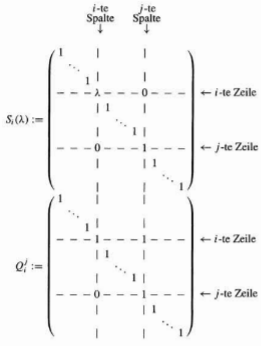
\includegraphics[width= 0.48\textwidth]{pics/ElMa1.png} & 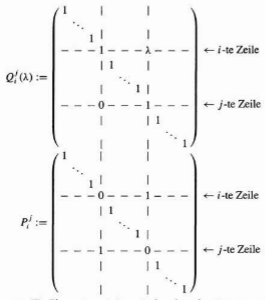
\includegraphics[width= 0.48\textwidth]{pics/ElMa2.png}
\end{tabular}
Die Matrizen $S_i(\lambda), Q^j_i, Q^j_i(\lambda)$ und $P^j_i$ heißen Elementarmatrizen. Analog mit Spaltenumformungen $(i\neq j)$: \begin{itemize}
\item $A\cdot S_i(\lambda)$ entsteht aus $A$ durch Multiplikation der $i$-ten Spalte mit $\lambda$.
\item $A\cdot Q^j_i(\lambda)$ entsteht aus $A$ durch Addition des $\lambda$-fachen der $i$-ten Spalte zur $j$-ten Spalte.
\item $A\cdot P^j_i$ entsteht aus $A$ durch Vertauschen der $i$-ten und $j$-ten Spalte.
\end{itemize}
\begin{Bemerkung}
Die Elementarmatrizen $(\lambda\neq 0)$ $Q^j_i(\lambda)$ und $P^j_i$ sind Produkte von Elementarmatrizen des Typs I und II, genauer : $Q^j_i(\lambda)=S_j(\frac{1}{\lambda})\cdot Q^j_i\cdot S_j(\lambda)$ bzw. $P^j_i=Q^i_j\cdot Q^j_i(-1)\cdot Q^i_j\cdot S_j(-1)$.
\end{Bemerkung}
\begin{Lemma}
Die Elementarmatrizen sind invertierbar und ihre Inverse sind auch Elementarmatrizen: $(S_i(\lambda))^{-1}=S_i(\frac{1}{\lambda})$, $(Q^j_i)^{-1}=Q^j_i(-1)$, $(Q_i^j(\lambda))^{-1}=Q^j_i(-\lambda)$ ,$(P^j_i)^{-1}=P^j_i$.
\end{Lemma}
\begin{Satz}
Jede invertierbare Matrix $A\in\emph{GL}(m,K)$ ist ein endliches Produkt von Elementarmatrizen. \glqq$\emph{GL}(m,K)$ wird von den Elementarmatrizen erzeugt.\grqq
\end{Satz}
\subsection{Rechenverfahren zur Bestimmung inverser Matrizen}
$A\in M(n\times n,K)$ quadratische Matrix
\begin{itemize}
\item Schreibe $E_n$ in eine Spalte neben $A$.
\item bringe $A$ durch Zeilenumformungen auf Zeilenstufenform; führe alle Zeilenumformungen parallel mit $E_n$ durch
\item Wenn Zeilenstufenform erreicht ist, lese ab, ob $A$ maximalen Rang hat. Falls rang$(A)<n$, dann ist $A$ nicht invertierbar und breche ab.
\item mache $A$ durch weitere Zeilenumformungen zur Einheitsmatrix $E_n$; wieder werden alle Umformungen parallel mit der zweiten Spalte gemacht.
\item am Ende steht rechts die inverse Matrix $A^{-1}$.
\end{itemize}
\begin{Bemerkung}
Das Verfahren funktioniert auch, wenn man ausschließlich Spaltenumformungen vornimmt. \underline{Warnung:} nicht Zeilen- und Spaltenumformungen mischen.
\end{Bemerkung}
Sei $A\in M(m\times n,K)$. Es gibt immer invertierbare Matrizen $S\in\text{GL}(m,K)$ und $T\in\text{GL}(n,K)$ mit $S\cdot A\cdot T^{-1}=\left(\begin{matrix} E_r & 0 \\ 0 & 0 \end{matrix}\right)$, wobei $r=\text{rang}(A)$.
\subsection{Gauß-Verfahren mit Elementarmatrizen}
Gegeben $A\in M(m\times n,K)$ und $b\in K^m$, gerade ist Lös$(A,b)=\{x\in K^n:Ax=b\}$. Es gibt $S\in $ GL$(m,K)$, Produkt von Elementarmatrizen, sodass $S\cdot A$ Zeilenstufenform hat. Setze $\tilde{A}=S\cdot A, \tilde{b}=S\cdot b$, dann gilt Lös$(A,b)=\text{Lös}(S\cdot A, S\cdot b)=\text{Lös}(\tilde{A},\tilde{B})$. An $(\tilde{A},\tilde{B})$ kann man ablesen, ob es Lösungen gibt: Falls $\tilde{b_i}\neq 0$ für $i>\text{rang}(A) \Rightarrow \text{Lös}(A,b)=\emptyset$
\section{Determinanten}
\subsection{Beispiele und Definitionen}
\begin{bez}
Ist $A$ quadratische Matrix mit $n$ Zeilen, so beizeichnen wir mit $a_1,...,a_n$ die Zeilenvektoren von $A$. Dann schreiben wir
\[A=\begin{pmatrix} a_1\\\vdots\\a_n\end{pmatrix}\]
\end{bez}
\begin{Definition}
Sei $K$ Körper und $n$ natürliche Zahl ungleich Null. Eine Abbildung
$\operatorname{det}\colon M(n\times n,K)\rightarrow K, A\mapsto \operatorname{det} (A)$
heißt \herv{Determinante}, falls folgendes gilt:
\begin{enumerate}
\renewcommand{\labelenumi}{\emph{\underline{D\arabic{enumi}}}}
\item $\operatorname{det}$ ist \herv{linear} in jeder Zeile, d.h. für alle $i\in\{1,...,n\}$ gilt:\begin{enumerate}
\renewcommand{\labelenumi}{\emph{(\alph{enumi})}}
\item  Ist $a_i=a_i'+a_i''$, so ist
\[\operatorname{det}\begin{pmatrix} \vdots\\ a_i\\\vdots\end{pmatrix}=\operatorname{det}\begin{pmatrix} \vdots\\ a_i'\\\vdots\end{pmatrix}+\operatorname{det}\begin{pmatrix} \vdots\\ a_i''\\\vdots\end{pmatrix}.\]
\item  Ist $a_i=\lambda a_i'$, so ist
\[\operatorname{det}\begin{pmatrix} \vdots\\ a_i\\\vdots\end{pmatrix}=\lambda\operatorname{det}\begin{pmatrix} \vdots\\ a_i'\\\vdots\end{pmatrix}.\]
\end{enumerate}
\item $\operatorname{det}$ ist \herv{alternierend}, d.h. hat $A$ zwei gleiche Zeilen, so ist $\operatorname{det} (A)=0$.
\item $\operatorname{det}$ ist \herv{normiert}, d.h. $\operatorname{det} (E_n)=1$.
\end{enumerate}
\end{Definition}
Man schreibt die Determinante auch folgendermaßen: Sei $A=(a_{ij})$ quadratische Matrix mit $n$ Zeilen. Dann ist
\[\left\lvert\begin{matrix}a_{11}&a_{12}& \ldots &a_{1n}\\ a_{21}&a_{22}&\ldots &a_{23}\\
\vdots & \vdots & \ddots & \vdots \\a_{m1}&a_{m2}&\ldots & a_{mn}\end{matrix}\right\rvert :=\lvert A\rvert :=\det(A).\]
Alles, was im folgenden nur für Zeilen gemacht wird, kann auch genauso mit Spalten gemacht werden. Das ist eine unmittelbare Konsequenz aus $\det (A)=\det(\presuper t A)$.
\begin{Satz}
Sei $\det\colon M(n\times n;K)\rightarrow K$ eine Determinante, $A\in M(n\times n;K)$. Dann gelten:
\begin{enumerate}
\setcounter{enumi}{3}
\renewcommand{\labelenumi}{\emph{\underline{D\arabic{enumi}}}}
\item $\forall \lambda\in K\colon \det (\lambda A)=\lambda^n\det (A)$.
\item Ist eine Zeile von $A$ gleich Null, so ist $\det (A)=0$.
\item Die Determinante ändert bei Zeilenumformungen vom Typ IV (Vertauschen zweier Zeilen) ihr Vorzeichen.
\item Die Determinante bleibt bei Zeilenumformungen vom Typ III (Addition des Vielfachen einer Zeile zu einer anderen Zeile) unverändert.
\item Ist $A$ obere Dreiecksmatrix mit Diagonaleinträgen $\lambda_1,...,\lambda_n$, so ist $\det(A)=\lambda_1\cdot...\cdot\lambda_n$.
\item Ist $A$ von der Form
\[A=\begin{pmatrix} A_1&C\\0&A_2\end{pmatrix},\]
wobei $A_1,A_2$ quadratisch sind und mindestens eine Zeile haben, dann gilt
$\det (A)=\det (A_1)\cdot \det(A_2).$
\item $\det (A)=0$ gdw. $\operatorname{rang} A<n \Leftrightarrow ( \det(A) \neq 0 \Leftrightarrow\text{ A invertierbar})$.
\item Sei $B\in M(n\times n;K)$. Dann gilt
$\det(AB)=\det (A)\cdot\det (B)$.
Daraus folgt sofort
$\det(A^{-1})=\det(A)^{-1}$.
(Hinweis: Im Allgemeinen gilt nicht $\det(A+B)=\det(A) +\det(B)$.)
\end{enumerate}
\end{Satz}
Bei der Berechnung von Determinanten bringt man die Matrix mit elementaren Zeilenumformungen (D$7$) auf Dreiecksgestalt und merkt sich dabei, wie oft man Zeilen mit Skalaren multipliziert hat (D$1$(b)) und wie oft man Zeilen vertauscht hat (D$6$). Dann wendet man D$8$ an.
\subsection{Existenz und Eindeutigkeit}
\begin{Definition}
Sei $n\in\mathbb N$. \herv{$S_n$} ist die symmetrische Gruppe, d.h. die Gruppe aller Bijektionen
$\sigma\colon \{1,...,n\}\rightarrow \{1,..,n\}$
mit der Komposition als Multiplikation. Diese Bijektionen heißen Permutationen. Das neutrale Element der $S_n$ ist $id$, die Identität.
\end{Definition}
\begin{Bemerkung}
\[\lvert S_n\rvert=n!\]
Ferner ist $S_n$ für $n\geq 3$ nicht kommutativ.
\[n!\approx \sqrt{2\pi n}\left(\frac n e\right)^n\]
(Diese Formel ist vermutlich nicht klausurrelevant.)
\end{Bemerkung}
\begin{Definition}
$\tau\in S_n$ heißt \herv{Transposition}, wenn $\tau$ genau zwei Elemente aus $\{1,\ldots ,n\}$ vertauscht und alle anderen fest lässt. Formal: Sei $\tau\in S_n$. Dann
$\tau \text{ ist Transposition gdw. }\exists k,l\in\{1,...,n\}\colon k\neq l, \tau(k)=l,\tau(l)=k,\tau(i)=i\forall i\in\{1,...,n\}\setminus\{k,l\}$
\end{Definition}
\begin{Bemerkung}
Für jede Transposition $\tau$ gilt $\tau=\tau^{-1}$.
\end{Bemerkung}
\begin{Lemma}
Für $n\geq 2$ lässt sich jede Permutation als Komposition von endlich vielen Transpositionen schreiben.
\end{Lemma}
\begin{Bemerkung}
Sei $\tau_0=(12)$. Für alle Transpositionen $\tau\in S_n$ existiert dann ein $\sigma\in S_n$ mit
\[\tau=\sigma\circ\tau_0\circ\sigma^{-1}\]
\end{Bemerkung}
\begin{Definition}
Ist $\sigma\in S_n$, so heißt jedes Paar $i,j\in\{1,...,n\}$ mit
\[i<j, \sigma(i)>\sigma(j)\]
\herv{Fehlstand} von $\sigma$.
Das \herv{Signum} von $\sigma$ ist definiert durch
\[\operatorname{sign}\sigma:=\left\{\begin{array}{ll} +1, &\text{falls }\sigma\text{ eine gerade Anzahl von Fehlständen hat,}\\ -1,&\text{falls } \sigma \text{ eine ungerade Anzahl von Fehlständen hat.}\end{array}\right.\]
Man nennt $\sigma$ gerade, falls $\operatorname{sign}\sigma=+1$, und sonst ungerade.
\end{Definition}
\begin{Lemma}
Für jedes $\sigma\in S_n$ gilt
$\operatorname{sign}\sigma = \prod_{i<j}\frac{\sigma(j)-\sigma(i)}{j-i}$
\end{Lemma}
\begin{Satz}
Für alle Permutationen $\sigma,\tau$ gilt $\operatorname{sign}(\tau\circ\sigma)=\operatorname{sign}(\tau)\cdot\operatorname{sign}(\sigma)$.
\end{Satz}
\begin{Korollar}
Sei $n\geq 2$.
\begin{enumerate}
\renewcommand{\labelenumi}{\emph{\arabic{enumi})}}
\item Für jede Transposition $\tau$ gilt $\operatorname{sign}(\tau)=-1$.
\item Ist $\sigma\in S_n$ und $\sigma=\tau_1\circ...\circ\tau_k$ mit Transpositionen $\tau_1,...,\tau_k\in S_n$, so ist $\operatorname{sign}\sigma=(-1)^k$
\end{enumerate}
\end{Korollar}
\begin{Korollar}
Für jede Permutation $\sigma\in S_n$ ist
\[\det\begin{pmatrix} e_{\sigma(1)}\\\vdots\\e_{\sigma(n)}\end{pmatrix}=\operatorname{sign}\sigma\]
\end{Korollar}
\begin{Definition}
Man kann eine Äquivalenzrelation auf der symmetrischen Gruppe $S_n$ definieren, in denen zwei Permutationen genau dann äquivalent sind, wenn sie dasselbe Signum besitzen. Die Äquivalenzklassen sind dann die geraden und die ungeraden Permutationen. Die geraden Permutationen bilden eine Untergruppe von der symmetrischen Gruppe und wird auch die \herv{alternierende Gruppe} $A_n$ genannt. Ist $\tau$ eine ungerade Permutation, so kann die Menge der ungeraden Permutationen als $A_n \tau:=\{\sigma\circ\tau\colon\sigma\in A_n\}$ geschrieben werden.
\end{Definition}
\begin{Bemerkung}
Sei $\tau\in S_n$ eine ungerade Permutation. Dann ist $S_n=A_n\cup A_n\tau\ und\ A_n\cap A_n\tau=\emptyset$.
Insbesondere hat $A_n$ genau $\frac{n!}2$ Elemente für alle $n\geq 2$.
\end{Bemerkung}
\begin{Theorem}
Sei $K$ ein Körper, $n\geq 1$, so gibt es genau eine Determinante
$\det\colon M(n\times n;K)\rightarrow K,$
und zwar ist für $A=(a_{ij})\in M(n\times n;K)$
\[\det(A)=\sum_{\sigma\in S_n} \operatorname{sign}(\sigma)\cdot a_{1\sigma(1)}\cdot...\cdot a_{n\sigma(n)}\]
Diese Formel wird auch Leibniz-Formel genannt.
\end{Theorem}
\begin{Bemerkung}
Für $K=\R$ und $K=\C$ ist die Determinantenfunktion differenzierbar und insbesondere stetig.
\end{Bemerkung}
\begin{Satz}
Sei $A$ eine quadratische $n\times n$-Matrix über dem Körper $K$. Dann gilt $\det(\presuper tA)=\det(A)$.
\end{Satz}
\begin{Bemerkung}
Die Formel $\det(A)=\sum_{\sigma\in S_n} {\operatorname{sign}(\sigma)\cdot a_{1\sigma(1)}\cdot \ldots \cdot a_{n\sigma(n)}}$ definiert eine Funktion für $n\times n$-Matrizen über jeden kommutativen Ring $R$ mit $1$ $\det: M(n\times n,R)\rightarrow R$. Die Eigenschaften D$1$, D$2$ und D$3$ gelten. Außerdem alle weiteren, in deren Beweis nicht dividiert wurde.
\end{Bemerkung}
\begin{Beispiel}
Die \textbf{Vandermonde-Determinate} ist \[K[x_1,\ldots,x_n]\ni\Delta_n=\left|\begin{matrix}
1 & x_1 & x_1^2 & \ldots & x_1^{n-1} \\
1 & x_2 & x_2^2 & \ldots & x_2^{n-1} \\
\vdots & \vdots & \vdots & \ddots & \vdots \\
1 & x_n & x^2_n & \ldots & x_n^{n-1}
\end{matrix} \right|=\prod_{1\leq i < j \leq n} (x_j-x_i) .\] (lässt sich über Induktion zeigen)
\end{Beispiel}
\begin{Korollar}
Seien $x_1,\ldots,x_n\in K$. Dann ist die Vandermonde-Matrix genau dann invertierbar, wenn $x_1,\ldots,x_n$ paarweise verschieden sind.
\end{Korollar}
\subsection{Minoren}
\begin{Definition}
Sei $A\in M(n\times n,K)$. Für $i,j\in\{1,\ldots,n\}$ entstehe $A_{ij}\in M(n\times n,K)$ aus A, indem $a_ij$ durch $1$ ersetzt wird und alle anderen Einträge der $i$-ten Zeile und $j$-ten Spalte zu $0$ gesetzt werden. Die \herv{komplementäre Matrix} $A^\#=(a_{ij}^\#)\in M(n\times n, K)$ ist definiert durch $a_{ij}^\#=\det(A_{ji})$. 
\end{Definition}
\begin{Satz}
Es gilt $A\cdot A^\#=A^\#\cdot A=\det(A)\cdot E_n$.
\end{Satz}
\begin{Definition}
Es entstehe $A'_{ij}\in M((n-1)\times(n-1);K)$ aus A durch Streichen der i-ten Zeile und j-ten Spalte.
\end{Definition}
\begin{Bemerkung}
$\det(A_{ij})=(-1)^{i+j}\det(A'_{ij})$
\end{Bemerkung}
\begin{Bemerkung}
Es gilt $\det(A_{ij})=\det(a^1,a^2,\ldots,a^{j-1},e^{i},a^{j+1},\ldots,a^n)$, wobei $a^k$ die $k$-te Spalte von $A$ ist und $e^i=\presuper t {(e_i)}$
\end{Bemerkung}
\begin{Korollar}
Eine Matrix $A\in M(n\times n, R)$ ist genau dann invertierbar, falls $\det(A)$ eine Einheit in R ist, also ein inverses Element bezüglich $\cdot$ hat. (R ist Ring).
\end{Korollar}
\begin{Satz}[Entwicklungssatz nach Laplace]
Für alle $A\in M(n\times n, K)$ gilt:\begin{itemize}
\item für alle $i\in \{1,\ldots,n\}$ gilt $\det(A)=\sum_{j=1}^n{(-1)^{i+j}a_{ij}\cdot \det(A'_{ij})}$ \glqq Entwicklung nach der i-ten Zeile.\grqq
\item für alle $j\in \{1,\ldots,n\}$ gilt $\det(A)=\sum_{i=1}^n{(-1)^{i+j}a_{ij}\cdot \det(A'_{ij})}$ \glqq Entwicklung nach der j-ten Zeile.\grqq
\end{itemize}
\end{Satz}
\begin{Satz}
Sei $A\in\emph{GL}(n,K)$ und definiere $C\in \emph{GL}(n,K)$ durch $c_{ij}=(-1)^{i+j}\cdot\det(A'_{ij})=\det(A_{ij})=a^\#_{ji}$. Dann gilt $A^{-1}=\frac{1}{\det(A)}\cdot \presuper tC$
\end{Satz}
Für $n=2$ gilt dies: $A^{-1}=\frac{1}{ad-bc}\cdot\left(\begin{matrix} d & -b \\ -c & a  \end{matrix}\right)$.
\begin{Bemerkung}
Für $A\in \text{GL}(n,K)$ hat jedes inhomogene Gleichungssystem $A\cdot x=b, x,b\in K^n$ eine eindeutige Lösung gegeben durch $x=\presuper t {(x_1,\ldots, x_n)}$ mit $x_i=\frac{\det(a^1,\ldots,a^{i-1},b,a^{i+1},\ldots,a^n)}{\det(A)}\in K$ für alle $i=1,\ldots,n$.
\end{Bemerkung}
\begin{Definition}
Sei $A\in M(m\times n, K)$ und $k\leq min\{m,n\}$. Eine Matrix $A'\in M(k\times k, K)$ heißt \herv{k-reihige Teilematrix} von A, falls sich A durch Zeilen- und Spaltenvertauschungen auf die Form $\left(\begin{matrix}
A' & * \\ * & * \end{matrix}\right)$ bringen lässt. (Streichen von Zeilen und Spalten zählt auch dazu). Der Skalar $\det(A')$ heißt ein \herv{k-reihiger Minor} von A.
\end{Definition}
\begin{Satz}
Sei $A\in M(m\times n, K)$ und $r\in \N$ mit $r\leq \min\{m,n\}$. Dann sind äquivalent: \begin{enumerate}
\renewcommand{\labelenumi}{\emph{(\roman{enumi})}}
\item $\emph{rang}(A)=r$
\item Es gibt einen r-reihigen Minor, der von $0$ verschieden ist, und für alle $k>r$ ist jeder k-reihige Minor gleich $0$.
\end{enumerate}
\end{Satz}
\begin{Definition}
Sei V ein endlichdimensionaler K-Vektorraum und $F:V\rightarrow V$ ein Endomorphismus. Die Determinante von $F$ ist definiert als $\det(F)=\det(M^\mathcal{B}_\mathcal{B}(F))$ für eine Basis $\mathcal{B}$ von V. Dies ist unabhängig von der Wahl der Basis $\mathcal{B}$.
\end{Definition}
\begin{Bemerkung}
Für $F\in\text{End}_K(V),\dim(V)<\infty$ sind äquivalent: 
\begin{enumerate}
\renewcommand{\labelenumi}{(\roman{enumi})}
\item $F$ ist injektiv.
\item $F$ ist surjektiv.
\item $F$ ist bijektiv.
\item $\det(F)\neq 0$.
\end{enumerate}
\end{Bemerkung}
\textbf{Ab hier ist $\mathbf{K=\R}$}
\begin{Definition}
Sei V ein endlichdimensionaler Vektorraum. Ein Automorphismus $F:V\rightarrow V$ heißt \begin{itemize}
\item \herv{orientierungstreu}, falls $\det(F)>0$
\item \herv{orientierungsuntreu}, falls $\det(F)<0$
\end{itemize}
Seien $\mathcal{A}=(v_1,\ldots,v_n)$ und $\mathcal{B}=(w_1,\ldots,w_n)$ zwei Basen eines $\R$-Vektorraums V. Sei $F:V\rightarrow V$ derjenige Automorphismus mit $F(v_i)=w_i$ für alle $i=1,\ldots,n$. $\mathcal{A}$ und $\mathcal{B}$ heißen \herv{gleichorientiert}, $A\sim B$, falls $\det(F)>0$.
\end{Definition}
\begin{Bemerkung}
\glqq gleichorientiert \grqq\ ist eine Äquivalenzrelation auf der Menge aller Basen von $V$ mit genau $2$ Äquivalenzklassen. Eine \herv{Orientierung} von $V$ ist eine solche Äquivalenzklasse.
\end{Bemerkung}
Für $V=\R^n$ kann man eine Orientierung auszeichnen, nämlich die, die die kanonische Basis $K=(e_1,\ldots,e_n)$ enthält: $\{A:A\sim K\}=\{A=(v^1,\ldots,v^n):\det(v^1,\ldots,v^n)>0\}$ bzw. $\{A:A\not\sim K\}=\{A=(v^1,\ldots,v^n):\det(v^1,\ldots,v^n)<0\}$\\
Sei $G_+:=\{A\in \text{GL}(n,\R):\det(A)>0\}$, dies ist Untergruppe von $\text{GL}(n,\R)$.\\
$G_-:=\{A\in \text{GL}(n,\R):\det(A)<0\}$. Es gilt $\text{GL}(n,\R)=G_+\cup G_{-}$.
\begin{Bemerkung}
Sei $T\in \text{GL}(n,\R)$ und $\det(T)<0$. Dann sind $-\cdot T: G_{+}\rightarrow G_-$ und $-\cdot T^{-1} : G_-\rightarrow G_+$ zueinander inverse Bijektionen. Insbesondere $G_-=G_+\cdot T$. Also $\text{GL}(n,\R)=G_+\cup (G_+\cdot T), G_+\cap(G_+\cdot T)=\emptyset$.
\end{Bemerkung}
\begin{Definition}
Zwei Matrizen $A,B\in \emph{GL}(n,\R)$ heißen verbindbar, falls es eine stetige Abbildung $\varphi:[0;1]\rightarrow \emph{GL}(n,\R)$ gibt, mit $\varphi(0)=A, \varphi(1)=B$. ($\varphi$ heißt stetig, wenn jede der $n^2$ Koordinatenfunktionen stetig ist.)
\end{Definition}
\begin{Satz}
Für $A,B\in \emph{GL}(n,\R)$ sind äquivalent:
\begin{itemize}
\renewcommand{\labelenumi}{\emph{(\roman{enumi})}}
\item Es gilt $\det(A\cdot B)>0$ (oder äquivalent: A und B liegen in derselben Klasse von $\emph{GL}(n,\R)=G_+\cupdot G_-$)
\item A und B sind in $\emph{GL}(n,\R)$ verbindbar.
\end{itemize}
\end{Satz}
\begin{Lemma}
Sei $A\in \emph{GL}(n,\R)$ mit $\det(A)>0$. Dann ist A mit $E_n$ verbindbar.
\end{Lemma}
\end{document}